\documentclass[conference]{IEEEtran}
\usepackage{amsmath}
\usepackage{amsfonts}
\usepackage{forest}
\usepackage{tikz}
\usetikzlibrary{automata,positioning}
\usetikzlibrary{arrows,automata}
\usepackage{adjustbox}
\usepackage{lipsum}
\usepackage{mathtools}
\usepackage{paralist}
\DeclarePairedDelimiter{\ceil}{\lceil}{\rceil}
\usepackage{array}
\usepackage{eqparbox}
\usepackage{algorithm,algorithmic}

\usepackage{etoolbox}  % patch def of algorithmic environment
\usepackage{array}
\usepackage{eqparbox}
\renewcommand\algorithmiccomment[1]{%
	\hfill\#\ \eqparbox{COMMENT}{#1}%
}


\makeatletter
\newcounter{ALC@tempcntr}% Temporary counter for storage
\newcommand{\LCOMMENT}[1]{%
	\setcounter{ALC@tempcntr}{\arabic{ALC@rem}}% Store old counter
	\setcounter{ALC@rem}{1}% To avoid printing line number
	\item \# #1% Display comment + does not increment list item counter
	\setcounter{ALC@rem}{\arabic{ALC@tempcntr}}% Restore old counter
}%
\makeatother
%\usepackage{algorithm}

\usepackage{amsthm}
\newtheorem{theorem}{Theorem}[section]
\newtheorem{corollary}{Corollary}[theorem]
\newtheorem{lemma}[theorem]{Lemma}

\theoremstyle{definition}
\newtheorem{defn}{Definition}[section]


\newtheorem{example}{Example}
\newcommand{\mi}[1]{\mathit{#1}}
\newcommand{\sia}{\mi{S^a_i}}
\newcommand{\iia}{\mi{I^a_i}}
\newcommand{\aia}{\mi{A^a_i}}
\newcommand{\gia}{\mi{G^a_i}}
\newcommand{\tia}{\mi{T^a_i}}
\newcommand{\pia}{\mi{P^a_i}}
\newcommand{\hia}{\mi{H^a_i}}
\newcommand{\ahia}{\mi{AH^a_i}}
\newcommand{\shia}{\mi{SH^a_i}}
\newcommand{\gs}{S}
\newcommand{\sat}{\models}
\newcommand{\sib}{\mi{S^b_i}}
\newcommand{\iib}{\mi{I^b_i}}
\newcommand{\aib}{\mi{A^b_i}}
\newcommand{\tib}{\mi{T^b_i}}
\newcommand{\sir}{\mi{S^r_i}}
\newcommand{\iir}{\mi{I^r_i}}
\newcommand{\air}{\mi{A^r_i}}
\newcommand{\gir}{\mi{G^r_i}}
\newcommand{\tir}{\mi{T^r_i}}
\newcommand{\hir}{\mi{H^r_i}}
\newcommand{\ahir}{\mi{AH^r_i}}
\newcommand{\shir}{\mi{SH^r_i}}
\newcommand*\xor{\mathbin{\mi{xor}}}


\author{
    \IEEEauthorblockN{Fernando Dileepa\IEEEauthorrefmark{1}, Naipeng Dong\IEEEauthorrefmark{2}, Cyrille Jegourel\IEEEauthorrefmark{3}, Jin Song Dong\IEEEauthorrefmark{4}}
    \IEEEauthorblockA{National University of Singapore
    \\\{fdileepa\IEEEauthorrefmark{1}, dongnp\IEEEauthorrefmark{2}, jegourel\IEEEauthorrefmark{3}, dongjs\IEEEauthorrefmark{4}\}@comp.nus.edu.sg}
}
\begin{document}
\title{Verification of Nash-Equilibrium for Probabilistic BAR Systems}
\maketitle
\begin{abstract}
A BAR system specifies a cooperation between agents who can be altruistic when they follow the specified behaviours, Byzantine when they randomly deviate from specifications and rational when they deviate to increase their own benefits. We consider whether a rational agent indeed follows the specification of a probabilistic BAR system as verifying whether the system is a Nash-equilibrium in the corresponding stochastic games. In this article, we propose an intuitive specification for probabilistic BAR systems and an algorithm to automatically verify Nash-equilibrium. To validate our implementation of the algorithm, we present two case studies -- the three-player Rock-paper-scissors game and a probabilistic secret sharing protocol. 
\end{abstract}

\section{Introduction}
Game Theory is the study of mathematical models of conflict and cooperation between multiple agents who are considered as intelligent and rational decision-makers, and is used in a large range of domains (economics, psychology, computer science...). In communication networks, the protocols are seen as games in which the involved entities of the network must cooperatively follow the protocol rules. However, it may be possible that a particular entity is corrupted or does not work correctly with respect to the protocol. Some device may have been designed to deviate from the protocol to maximise a self-interest function or may be simply misconfigured. A protocol is unlikely to work correctly with respect to a property in the presence of selfish or ``broken" agents. However, it remains of first importance to guarantee some safety property under these conditions. For example, in the secret sharing protocol, we expect that a corrupted agent cannot reconstruct highly sensitive information before the other agents. Byzantine-Altruistic-Rational (BAR) models have been introduced in \cite{AACDMP05} in order to analyse the protocol correctness of systems under these conditions. In these systems, the agents are divided in three categories of players. They are said to be altruistic if they follow the rules of the protocol, even if a rational choice is to deviate from it. The agents are rational if they may deviate from the protocol in order to maximise their self-interest, captured in a utility function. Finally, Byzantine agents characterise the players who arbitrarily deviate from the protocol because of component failures, malicious intent, security compromise. The general architecture of BAR systems have been introduced in \cite{AACDMP05}. In the BAR framework, the correctness of the protocol with respect to some property is satisfied if the property remains true in spite of the presence of rational and Byzantine players. Such protocols are said BAR-tolerant. Some of them have been already proposed to implement cooperative services in peer-to-peer data streaming applications \cite{LCWNRAD06}.

BAR-tolerant protocols are thus important because, they guarantee that selfish agents actually play as expected by the protocol even if some agents are identified as broken or misconfigured. However, it remains challenging to prove that a protocol is BAR-tolerant. For that purpose, it is relevant to make use of Nash-equilibriums, a common game theory concept characterising strategies from which rational players should not deviate in order to maximise their utility. In \cite{MMSTACL08}, the authors presented a symbolic Model Checking algorithm that automatically verifies whether the proposed protocol is a \emph{Nash-equilibrium}. In \cite{Brenguier13}, PRALINE has been presented as a tool for computing Nash-equilibrium in non-probabilistic concurrent games played on graphs. By concurrent games, we mean games where the next state is defined at the beginning of a turn by the individual choices of all the players. However, these previous works are limited to non-\emph{probabilistic protocols}. Moreover, the game must be modelled with perfect information, meaning that the rational agents are assumed to have a perfect knowledge of the player utilities and of the global state of the game.

In our article, we focus on a particular class of probabilistic protocols, that is  protocols in which the agents take decisions accordingly to a specified probability distribution. The altruistic agents play thus with respect to this distribution, the rational agents play  with respect to the probability distribution that maximises their expected utility and the Byzantine agents play accordingly to any probability distribution. Note that we do not cover the case in which illegal decisions with respect to the BAR system may be taken by the rational and Byzantine players. Moreover, we consider probabilistic games in which the utilities are known by the rational agents, as well as the number of Byzantine players.

Related to our work, the tool PRISM-games \cite{CFKPS13} computes an optimal strategy for a coalition of rational players in a probabilistic game. This strategy can then be used to verify that the global strategy is a Nash-equilibrium. However, PRISM-games is limited to the analysis of turn-based games, that are games where agents select their moves in turns. Synchronisation between agents is thus not available directly in PRISM-games. Moreover, the protocols are with perfect information: the agents know the whole reward structure as well as the current global state of the game and the probability distributions of all the players. Finally, PRISM-games computes an optimal strategy up to some bounded number of iterations but it does not compute explicitly a potentially larger bound guaranteeing that a particular strategy is a Nash-equilibrium.

\subsection{Contributions and structure of the article}
In Section \ref{sec:spec}, we present the specification of parallel and synchronous probabilistic BAR systems. In Section \ref{sec:verification}, we propose a verification algorithm to verify Nash-equilibrium of the system. Finally, we apply the algorithm in two case studies, one with perfect information and one with imperfect information in Section \ref{sec:casestudy} and we present interesting results with regard of Byzantine agents. We summarise our results in Section \ref{sec:conclusion}. For the best of our knowledge, this is the first attempt of verifying Nash-equilibrium of probabilistic BAR systems. Nash-equilibrium is verified for imperfect information scenario as well as the perfect information scenario. This differs from previous works e.g.,~\cite{CFKPS13} and~\cite{MMSTACL08}, since we consider imperfect information games and since we verify Nash-equilibriums explicitly instead of approximate equilibriums \cite{CFKPS13}. Finally, our verification algorithm determines a bound for the number of iterations that guarantees the Nash-equilibrium property.    

%\section{Introduction}
Game Theory is the study of mathematical models of conflict and cooperation between multiple agents, considered as intelligent and rational decision-makers and is used in a large range of domains (economics, psychology, computer science...). In communication networks, the protocols are seen as games in which the involved entities of the network must cooperatively follow the protocol rules. However, it may be possible that a particular entity is corrupted or does not work correctly with respect to the protocol. Some device may have been designed to deviate from the protocol to maximise a self-interest function or may be simply misconfigured. In this article, we reason on Byzantine-Altruistic-Rational (BAR) models \cite{AACDMP05}. In these systems, the agents are divided in three categories of players. They are said to be altruistic if they follow the rules of the protocol, even if a rational choice is to deviate from it. The agents are rational if they may deviate from the protocol in order to maximise their self-interest, captured in a utility function. Finally, Byzantine agents characterise the players who arbitrarily deviate from the protocol because of component failures, malicious intent, security compromise. A general architecture of BAR systems have been introduced in \cite{AACDMP05}. In the BAR framework, the correctness of the protocol with respect to some property is satisfied if the property remains true in spite of the presence of rational and Byzantine players. Such protocols are said BAR-tolerant and some of them have already been proposed to implement cooperative services in peer-to-peer data streaming applications \cite{LCWNRAD06}.

BAR-tolerant protocols are thus important because they guarantee that selfish agents actually play as expected bythe protocol even if some agents are identified as broken or misconfigured. However, it remains challenging to prove that a protocol is BAR-tolerant. For that purpose, it is relevant to make use of Nash equilibriums, a common game theory concept characterising strategies from which rational players should not deviate in order to maximise their utility. in \cite{MMSTACL08}, the authors presented a symbolic Model Checking algorithm that automatically verifies whether the proposed protocol is a \emph{Nash-equilibrium}. In \cite{Brenguier13}, PRALINE has been presented as a tool for computing Nash equilibrium in non-probabilistic concurrent games played on graphs. By concurrent games, we mean games where the next state is defined at the beginning of a turn by the individual choices of all the players. However, these previous works are limited to non-\emph{probabilistic protocols}. Moreover, the game must be modelled with perfect information, meaning that the rational agents are assumed to have a perfect knowledge of the player utilities and of the global state of the game.

In our article, we focus on a a particular class of probabilistic protocols, that are protocols in which the agents take decisions accordingly to a specified probability distribution. The altruistic agents play thus with respect to this distribution, the rational agents play  with respect to the probability distribution that maximises their expected utility and the Byzantine agents play accordingly to any probability distribution. Note that we do not cover the case in which illegal decisions with respect to the protocol may be taken by the rational and Byzantine players. Moreover, we consider probabilistic games in which the utilities are known by the rational agents, as well as the number of Byzantine players.

Related to our work, the tool PRISM-games \cite{CFKPS13} computes an optimal strategy for one rational player in a probabilistic game with perfect information. This strategy can then be used to verify that the global strategy is a Nash-equilibrium. However, PRISM-games is limited to the analysis of turn-based games, that are games where agents select their moves in turns. Synchronisation is thus not available directly in PRISM-games.
%\section{Contributions}
For the best of our knowledge, this is the first attempt of modelling and verifying probabilistic BAR systems. 
\section{Specification}\label{sec:spec}

In BAR systems, the non-altruistic agents do not necessarily follow the protocol rules. It is thus necessary to capture their possible deviations through adequate specifications. Moreover, we consider probabilistic BAR systems. In this setting, the agents may have to choose a local action among several enabled actions. Their choices are governed by a probability distribution. In this section, we present a framework which allows us to formally specify a probabilistic BAR system as a game in an intuitive way. We highlight that our framework facilitates modelling of concurrent games with some imperfect information. In our case, we restrict the imperfect information for a player to the knowledge of her opponents' local states. It means that each agent knows her own local state, the entire reward structure of the game, as well as, given a global state, the outgoing probability distribution.

We first show the formal modelling of each type of players as Finite State Machines (FSM) and then depict the combination of the FSMs to form a global transition system modelling the global behaviour of the whole system.

\subsection{Altruistic players}\label{ssec:al}
Altruistic player's behaviours that are specified in a protocol, can be formally captured by a FSM defined as a tuple $\mathcal{M}^a_i=(\sia, \iia, \aia, \gia, \tia, \pia, \hia)$ where 
\begin{itemize}
\item $\sia$ is the (finite) set of states of altruistic player $i$, 
\item $\iia$ denotes the set of initial states, 
\item $\aia$ is the set of actions, 
\item $\gia$ is the set of atomic propositions defined on global states $\gs$ that serves as guard conditions of taking an action and gaining rewards,
\item $\tia: [\phi] \sia \times \aia  \rightarrow \sia$, with $\phi$ being a first-order logic formula over $\gia$, specifies the transitions between states and the condition $\phi$ that needs to be satisfied for taking this transition,
\item $\pia: \sia \times \aia \rightarrow [0, 1]$ such that $\forall s_i\in \sia, \sum_{a_i\in \aia} \pia(s_i, a_i)=1$ specifies the probabilities of taking an action at state $s_i$,
\item $\hia$ has two functions $\ahia: \sia \times \aia \rightarrow \mathbb{R}$ specifies the pay-off of an action $a_i\in \aia$ at state $s_i\in \sia$, and $\shia: [\phi]\gs \rightarrow \mathbb{R}$ specifies the pay-off obtained after reaching states $\gs$ satisfying formula $\phi$.
\end{itemize}
%
When the system is well-defined, altruistic players have either a probabilistic or a deterministic behaviour, that is, at state $s_i\in \sia$, there is either one action $a_i\in \aia$ or a set of probabilistic actions whose probabilities sum up to $1$. When the action is deterministic, the probability is omitted, since the probability is always $1$.

\begin{example}\textit{A three-player Rock-paper-scissors game}\label{ex:rps}
Consider a $3$-player machine-game version of Rock-paper-scissors derived from \cite{PH10}. We model playing rock, paper, and scissors as playing $0$, $1$, and $2$, respectively. We denote $(i,j,k)$ as the respective outcomes of players $p_1$, $p_2$ and $p_3$, denote $+$ as the operator for the addition modulo $3$ and denote $a = b \oplus c$ as $a = b$ or, exclusively, $a = c$. The pay-off of player $p_1$ for the outcome $(i, j, k)$ is $2$ if $j=k$ and $i = j + 1$ ($p_1$ wins uniquely), $1$ if $i=k\oplus j$ and $i-1 = (j\oplus k)$ (both $p_1$ and another player win), $-1$ if $i + 1=j\oplus k$ ($p_1$ loses to one player), $-2$ if $j=k$ and $j = i + 1$ ($p_1$ loses to both players), and $0$ if $i = j = k$ or $i+1=j\oplus k \land i-1=k\oplus j $ (no one wins and three players play the same, or $p_1$ wins one player but loses to another). Player $p_2$'s pay-off is similar to the pay-off of player $p_1$ after replacing $i,j,k$ by $j,k,i$ in player $p_2$'s pay-off conditions. Player $p_3$'s pay-off is the negatives of player $p_1$'s plus player $p_2$'s pay-off. %Note that the game is a zero-sum game. In the two-player zero-sum rock-paper-scissors game, playing uniformly, \emph{ie} with probability $1/3$, rock, paper or scissors is the unique Nash equilibrium of the game.
\end{example}

We model altruistic player's behaviour in Example~\ref{ex:rps} as follows.
\begin{itemize}
\item
$\sia=\{s^a_1, s^a_2, s^a_3, s^a_4\}$, $\iia=\{s^a_1\}$, $\aia=\{0,1,2,\mi{replay}\}$, 
\item
$\gia=\{i = j, j = k, i = j + 1, j = i + 1, i=k\oplus j, i-1 = (j\oplus k), i + 1=j\oplus k \}$,
\item
$\tia(s^a_1, 0) = s^a_2,
\tia(s^a_1, 1) = s^a_3,
\tia(s^a_1, 2) = s^a_4,\\
~[\phi]\tia(s^a_4,\mi{replay})= s^a_1,
~[\phi]\tia(s^a_3,\mi{replay})= s^a_1,\\
~[\phi]\tia(s^a_2,\mi{replay})= s^a_1,$\\
with $\phi=\neg\big((j=k \land i = j + 1) \vee (i=k\land j=i+1) \vee (i=j\land k=i+1)\big)$,
meaning that the game terminates when there is a unique winner, and continues otherwise,
\item 
$\pia(s^a_1, 0) = 1/3, \pia(s^a_1, 1)= 1/3, \pia(s^a_1, 2) = 1/3$, and action $\mi{replay}$ is deterministic,
\item 
$\shia(\gs)=\left\{\begin{array}{l}
2\ \mbox{if}\ \gs \sat (j=k \land i = j + 1)\\
1\ \mbox{if}\ \gs \sat (i=k\oplus j \land i-1 = (j\oplus k))\\
0\ \mbox{if}\ \gs \sat ((i = j = k)\vee \\
\hfill(i+1=j\oplus k \land i-1=k\oplus j))\\
-1\ \mbox{if}\ \gs \sat (i + 1=j\oplus k)\\
-2\ \mbox{if}\ \gs \sat (j=k \land j = i + 1).\\
\end{array}\right. $
\end{itemize}


\subsection{Byzantine players}
Byzantine players may randomly deviate from the protocol by 1) performing actions that are not specified in the protocol, or 2) performing a set of probabilistic actions with a different probabilistic distribution. The deviating actions at a state shall be specified by the BAR system. As we want to ensure the BAR-tolerance of protocols, we only consider the worst-case scenario for the rational players, meaning that we assume that the Byzantine players always perform an action that minimizes the pay-off of the rational player. This action is unique, for that any distribution over the actions would not minimise the rational player's pay-off larger than one single action. Hence, there is no probability distribution needed for Byzantine players. In addition, since Byzantine players randomly deviate, the guard conditions and pay-off function are not needed neither.

Similar to the altruistic player, a Byzantine player can be formally modelled by a FSM, a tuple $\mathcal{M}^b_i=(\sib, \iib, \aib, \tib)$, where
\begin{itemize}
\item $\sib$ is the (finite) set of states of Byzantine player $i$, 
\item $\iib$ denotes the set of initial states, 
\item $\aib$ is the set of actions, 
\item $\tib: \sib \times \aib \rightarrow \sib$ specifies the transitions between states.
\end{itemize}

Assume that the Byzantine players in Example~\ref{ex:rps} can only deviate from the specification by playing according to a different probability distribution than the uniform distribution. A Byzantine player is modelled as follows:
\begin{itemize}
\item
$\sib=\{s^b_1, s^b_2, s^b_3, s^b_4\}$, $\iib=\{s^b_1\}$, $\aib=\{0,1,2, \mi{replay}\}$, 
\item
$\tib(s^b_1, 0) = s^b_2,
\tib(s^b_1, 1) = s^b_3,
\tib(s^b_1, 2) = s^b_4,\\
\tib(s^b_4,\mi{replay})= s^b_1,
\tib(s^b_3,\mi{replay})= s^b_1,\\ 
\tib(s^b_2,\mi{replay})= s^b_1.$\\
\end{itemize}

\subsection{Rational players}
Similar to Byzantine players, the rational players may also deviate from the protocol specification. Unlike Byzantine players, whose actions are random, the rational players' actions are driven by pay-offs, that is, at a state, the rational players choose the action that leads to larger pay-off. Similarly to the Byzantine players, this action is unique. In fact, a rational player has the same allowed transitions, states and actions as a Byzantine player. Unlike to the Byzantine players, the rational players need the pay-off function. Hence, a rational player can be formally modelled by a FSM, a tuple $\mathcal{M}^r_i=(\sir, \iir, \air, \gir, \tir, \hir)$, where
\begin{itemize}
\item $\sir$ is the (finite) set of states of rational player $i$, 
\item $\iir$ denotes the set of initial states, 
\item $\air$ is the set of actions, 
\item $\gir$ is the set of atomic propositions defined on global states $\gs$ that serves as guard conditions of gaining rewards,
\item $\tir: \sir \times \air \rightarrow \sir$ specifies the transitions between states,
\item $\hir$ has two functions: $\ahir:\sir \times \air \rightarrow \mathbb{R}$ specifies the pay-off of an action $a_i\in \air$ at state $s_i\in \sir$, and $\shir: [\phi]\gs \rightarrow \mathbb{R}$ specifies the pay-off of reaching states $\gs$ satisfying formula $\phi$.
\end{itemize}

A rational player in Example~\ref{ex:rps} is modelled as follows:
\begin{itemize}
\item
$\sir=\{s^r_1, s^r_2, s^r_3, s^r_4\}$, $\iir=\{s^r_1\}$, $\air=\{0,1,2, \mi{replay}\}$, 
\item
$\tir(s^r_1, 0) = s^r_2,
\tir(s^r_1, 1) = s^r_3,\\
\tir(s^r_1, 2) = s^r_4,
\tir(s^r_4,\mi{replay})= s^r_1,\\
\tir(s^r_3,\mi{replay})= s^r_1, 
\tir(s^r_2,\mi{replay})= s^r_1,$
\item
$\gir=\gia$,
\item 
$\shir(\gs)=\left\{\begin{array}{l}
2\ \mbox{if}\ \gs \sat (j=k \land i = j + 1)\\
1\ \mbox{if}\ \gs \sat (i=k\oplus j \land i-1 = (j\oplus k))\\
0\ \mbox{if}\ \gs \sat (i = j = k)\vee \\
\hfill(i+1=j\oplus k \land i-1=k\oplus j))\\
-1\ \mbox{if}\ \gs \sat (i + 1=j\oplus k)\\
-2\ \mbox{if}\ \gs \sat (j=k \land j = i + 1).\\
\end{array}\right. $
\end{itemize}

\subsection{Global graph}

Given a finite set of players 
%Byzantine players ($p_1,\ldots, p_m$), a finite set of players ($p_{m+1},\ldots, p_{n}$) who can behave as either rational or altruistic, 
modelled as FSMs ($\{\mathcal{M}_1, \ldots, \mathcal{M}_n\}$), one can construct a global
FSM $\mathcal{M}=(S, I, A, G, T, P, H)$ modelling the concurrent execution of player's FSMs.
Note that in our algorithm, the global graph is constructed implicitly on-the-fly. 
For the clearer presentation of our verification in the next section, we explicitly construct a global graph here
to provide an intuition on how a global graph is constructed.

%$\mathcal{M}_i=(S_i, I_i, A_i, G_i, T_i, P_i, H_i)$
%if $i \le m$ then $M_i=M^b_i$. Else ${M}_i={M}^a_i$ or ${M}_i={M}^r_i$. 
The global states in the global FSM is the product of the local states of each player, 
i.e., $S= S_1 \times S_2 \times\cdots\times S_n$; the set of initial states is 
$I = I_1 \times I_2 \times\cdots \times I_n$; the set of global actions 
is $A=$ $A_1 \times A_2 \times \cdots\times A_n$; the set of atomic propositions
is $G= G_1\cup G_2\cup \cdots\cup G_n$ ($G_i$ is empty if $\mathcal{M}_i$ models a Byzantine player).
%If $i \le m$ then $G_i = \phi$ for the completeness of the global graph.

Intuitively, the transition function $T$ is defined as
$T(\langle s_1,\ldots, s_n\rangle, \langle a_1, \ldots, a_n\rangle)=\langle s'_1 \ldots, s'_n\rangle$
where $T_i(s_i, a_i)=s'_i$ in $\mathcal{M}_i$ meaning that
at state $\langle s_1,\ldots, s_n\rangle$ every player takes an action according
to their local FSMs, then there is a transition in the global FSM. Note that we require
that every player has to take an action: Altruistic players always follow the protocol specification to take an action;
Byzantine and rational players may deviate from the specification by doing nothing or taking other actions, where
the deviation actions, including doing nothing, shall be defined and modelled in the local FSMs. 
We emphasize that we model each player's local actions rather than
requiring the global FSM as input like in~\cite{MMSTACL08}. Hence, we need to additionally consider the 
special cases where multiple users need to take actions at the same time, i.e., action synchronization,
e.g., in Example~\ref{ex:rps}, three players need to take the $\mi{replay}$ action at the same time, in order
to re-start the game. We support two ways of modelling synchronized actions: one
is to model action as one name with an arity, (\emph{e.g.} the number of players), such that more than the arity number of players taking the action can be synchronized, \emph{e.g.}, 
the $\mi{replay}/3$ means that at least three players want to re-start the game;
the other is to define a pair of actions, for example $(\mi{send}, \mi{receive})$ in communication,
meaning that whenever there is a $\mi{send}$ action and a $\mi{receive}$ action are enabled at a state,
the synchronized action can be taken. The synchronized actions need to be tagged in a
set $A_s$. Given a global action $\langle a_1, \ldots, a_n\rangle$, let $J(a)$ be defined as \\
$\forall a/arity \in A_s$, $J(a) \subset \{1, \dots ,n\}$ s.t. $\forall j \in J(a)$ $a_j=a$ with $|J(a)|=arity$. $J(a)$ specifies the exact set of positions that the synchronised action $a/arity$ can be activated.

In Example~\ref{ex:rps}, $A_s=\{\mi{replay}/3\}$. When an action $\langle a_1, \ldots, a_n\rangle$ 
is enabled at a state $s_i$, if $a_i$ is in $A_s$, but there is no other action to synchronize with, for the simplicity 
of modelling, we assume a failure state $s_f$ exists and $T(s, \langle a_1, \ldots, a_n\rangle)=s_f$. 
 Formally,
$T(s, \langle a_1, \ldots, a_n\rangle)=s_f$, if 
$\exists a/arity \in A_s$ s.t. $0 < |J(a)| < n$.
%$|\{a|a\in \{a_1,\ldots, a_n\}\land a/arity \in A_s\}|< arity$ or
%$(a,b) \in A_s \land (|\{a|a\in \{a_1,\ldots, a_n\}|\neq |\{b|b\in \{a_1,\ldots, a_n\}|)$, 
where $|A|$ denotes the number of elements in set $A$.

Generally, the probabilistic function is 
$P(\langle s_1,\ldots, s_n\rangle, \langle a_1, \ldots, a_n\rangle))=P_1(s_1, a_1) \times \ldots \times P_n(s_n, a_n)$.
If $P_i(s_i, a_i)$ is not defined i.e., in the case of deterministic or non-deterministic actions, we set the probability value to be $1$.
It is straightforward in the case that $a_i$ is a deterministic action. In the case of non-deterministic actions, once $a_i$ is chosen, it becomes deterministic, and thus the value is also $1$. 
In such a way, the probability of the global action $\langle a_1, \ldots, a_n\rangle$ at state $\langle s_1,\ldots, s_n\rangle$ 
i.e., $\prod_{i=1}^{n}P_i(s_i, a_i)$, actually captures the product of the probabilities of actions in $\{a_1, \ldots, a_n\}$,
and thus the probabilities of all global actions at a state sum up to $1$. When no action is probabilistic in the global 
action $\langle a_1, \ldots, a_n\rangle$, then we do not sign a probability to the action at the state, denoted as $P(\langle s_1,\ldots, s_n\rangle, \langle a_1, \ldots, a_n\rangle))=\circ$, meaning the probability is not defined.

The pay-off function $AH$ is defined as
$H(s,\langle a_1,\ldots, a_n\rangle)=\langle H_1(s,a_1), \ldots, H_n(s,a_n)\rangle$
where $H_i(s,a_i)$ can be empty, denoted as $\star$, meaning that function $H_i$
is not defined for action $a_i$ at state $s$. Similarly, $SH$ can be defined as,
$H(\langle s_1,\ldots, s_n\rangle)=\langle H_1(s_1), \ldots, H_n(s_n)\rangle$.

Given one altruistic player, one Byzantine player, one rational player, the 
global FSM for Example~\ref{ex:rps} is constructed using the above way. Since
there are too many states in the global FSM, we only demonstrate some interesting parts of the global FSM, for example, we only show the 
states with incoming and outgoing transitions.
\begin{itemize}
\item $S=\{\langle s^a_1, s^b_1, s^r_1 \rangle, \langle s^a_2, s^b_2, s^r_2 \rangle, 
\langle s^a_3, s^b_2, s^r_2\rangle, \langle s^a_2, s^b_3, s^r_2\rangle, \\
\langle s^a_2, s^b_2, s^r_3\rangle, \langle s^a_3, s^b_3, s^r_2 \rangle,\langle s^a_3, s^b_2, s^r_3 \rangle,\langle s^a_2, s^b_3, s^r_3 \rangle,\\
\langle s^a_3, s^b_3, s^r_3 \rangle, \langle s^a_4, s^b_2, s^r_2\rangle,
\langle s^a_2, s^b_4, s^r_2\rangle, \langle s^a_2, s^b_2, s^r_4\rangle,\\
\langle s^a_4, s^b_4, s^r_2\rangle, \langle s^a_4, s^b_2, s^r_4\rangle,
\langle s^a_2, s^b_4, s^r_4\rangle, \langle s^a_4, s^b_4, s^r_4\rangle,\\
\langle s^a_3, s^b_4, s^r_4\rangle, \langle s^a_4, s^b_3, s^r_4\rangle,
\langle s^a_4, s^b_4, s^r_3\rangle, \langle s^a_3, s^b_3, s^r_4\rangle,\\
\langle s^a_3, s^b_4, s^r_3\rangle, \langle s^a_4, s^b_3, s^r_3\rangle
\}$,
\item $I=\{\langle s^a_1, s^b_1, s^r_1 \rangle\}$,
\item $A=\{\langle a_1, a_2, a_3 \rangle | a_1, a_2, a_3 \in \{0,1,2, \mi{replay}\}$ and $A_s=\{\mi{replay}/3\}$,
\item $G=\gia$,
\item 
The playing transitions are:\\
$T(\langle s^a_1, s^b_1, s^r_1 \rangle, \langle 0, 0, 0 \rangle)=\langle s^a_2, s^b_2, s^r_2\rangle$,\\
$T(\langle s^a_1, s^b_1, s^r_1 \rangle, \langle 1, 0, 0\rangle)=\langle s^a_3, s^b_2, s^r_2\rangle$, \\
$T(\langle s^a_1, s^b_1, s^r_1 \rangle, \langle 0, 1, 0\rangle)=\langle s^a_2, s^b_3, s^r_2\rangle$, \\
$T(\langle s^a_1, s^b_1, s^r_1 \rangle, \langle 0, 0, 1\rangle)=\langle s^a_2, s^b_2, s^r_3\rangle$, \\
$T(\langle s^a_1, s^b_1, s^r_1 \rangle, \langle 1, 1, 0\rangle)=\langle s^a_3, s^b_3, s^r_2\rangle$, \\
$T(\langle s^a_1, s^b_1, s^r_1 \rangle, \langle 1, 0, 1\rangle)=\langle s^a_3, s^b_2, s^r_3\rangle$, \\
$T(\langle s^a_1, s^b_1, s^r_1 \rangle, \langle 0, 1, 1\rangle)=\langle s^a_2, s^b_3, s^r_3\rangle$, \\
$T(\langle s^a_1, s^b_1, s^r_1 \rangle, \langle 1, 1, 1\rangle)=\langle s^a_3, s^b_3, s^r_3\rangle$, \\
$T(\langle s^a_1, s^b_1, s^r_1 \rangle, \langle 2, 0, 0\rangle)=\langle s^a_4, s^b_2, s^r_2\rangle$, \\
$T(\langle s^a_1, s^b_1, s^r_1 \rangle, \langle 0, 2, 0\rangle)=\langle s^a_2, s^b_4, s^r_2\rangle$, \\
$T(\langle s^a_1, s^b_1, s^r_1 \rangle, \langle 0, 0, 2\rangle)=\langle s^a_2, s^b_2, s^r_4\rangle$, \\
$T(\langle s^a_1, s^b_1, s^r_1 \rangle, \langle 2, 2, 0\rangle)=\langle s^a_4, s^b_4, s^r_2\rangle$, \\
$T(\langle s^a_1, s^b_1, s^r_1 \rangle, \langle 2, 0, 2\rangle)=\langle s^a_4, s^b_2, s^r_4\rangle$, \\
$T(\langle s^a_1, s^b_1, s^r_1 \rangle, \langle 0, 2, 2\rangle)=\langle s^a_2, s^b_4, s^r_4\rangle$, \\
$T(\langle s^a_1, s^b_1, s^r_1 \rangle, \langle 2, 2, 2\rangle)=\langle s^a_4, s^b_4, s^r_4\rangle$, \\
$T(\langle s^a_1, s^b_1, s^r_1 \rangle, \langle 1, 2, 2\rangle)=\langle s^a_3, s^b_4, s^r_4\rangle$, \\
$T(\langle s^a_1, s^b_1, s^r_1 \rangle, \langle 2, 1, 2\rangle)=\langle s^a_4, s^b_3, s^r_4\rangle$, \\
$T(\langle s^a_1, s^b_1, s^r_1 \rangle, \langle 2, 2, 1\rangle)=\langle s^a_4, s^b_4, s^r_3\rangle$, \\
$T(\langle s^a_1, s^b_1, s^r_1 \rangle, \langle 1, 1, 2\rangle)=\langle s^a_3, s^b_3, s^r_4\rangle$, \\
$T(\langle s^a_1, s^b_1, s^r_1 \rangle, \langle 1, 2, 1\rangle)=\langle s^a_3, s^b_4, s^r_3\rangle$, \\
$T(\langle s^a_1, s^b_1, s^r_1 \rangle, \langle 2, 1, 1\rangle)=\langle s^a_4, s^b_3, s^r_3\rangle$,
\item
and the re-start transitions are:\\
$T(\langle s^a_2, s^b_2, s^r_2 \rangle, \langle \mi{replay},\mi{replay}, \mi{replay} \rangle)=\langle s^a_1, s^b_1, s^r_1\rangle$,\\
$T(\langle s^a_3, s^b_3, s^r_2 \rangle, \langle \mi{replay},\mi{replay}, \mi{replay} \rangle)=\langle s^a_1, s^b_1, s^r_1\rangle$,\\
$T(\langle s^a_3, s^b_2, s^r_3 \rangle, \langle \mi{replay},\mi{replay}, \mi{replay} \rangle)=\langle s^a_1, s^b_1, s^r_1\rangle$,\\
$T(\langle s^a_2, s^b_3, s^r_3\rangle, \langle \mi{replay},\mi{replay}, \mi{replay} \rangle)=\langle s^a_1, s^b_1, s^r_1\rangle$,\\
$T(\langle s^a_3, s^b_3, s^r_3\rangle, \langle \mi{replay},\mi{replay}, \mi{replay} \rangle)=\langle s^a_1, s^b_1, s^r_1\rangle$,\\
$T(\langle s^a_4, s^b_2, s^r_2\rangle, \langle \mi{replay},\mi{replay}, \mi{replay} \rangle)=\langle s^a_1, s^b_1, s^r_1\rangle$,\\
$T(\langle s^a_2, s^b_4, s^r_2\rangle, \langle \mi{replay},\mi{replay}, \mi{replay} \rangle)=\langle s^a_1, s^b_1, s^r_1\rangle$,\\
$T(\langle s^a_2, s^b_2, s^r_4\rangle, \langle \mi{replay},\mi{replay}, \mi{replay} \rangle)=\langle s^a_1, s^b_1, s^r_1\rangle$,\\
$T(\langle s^a_4, s^b_4, s^r_4\rangle, \langle \mi{replay},\mi{replay}, \mi{replay} \rangle)=\langle s^a_1, s^b_1, s^r_1\rangle$,\\
$T(\langle s^a_3, s^b_4, s^r_4\rangle, \langle \mi{replay},\mi{replay}, \mi{replay} \rangle)=\langle s^a_1, s^b_1, s^r_1\rangle$,\\
$T(\langle s^a_4, s^b_3, s^r_4\rangle, \langle \mi{replay},\mi{replay}, \mi{replay} \rangle)=\langle s^a_1, s^b_1, s^r_1\rangle$,\\
$T(\langle s^a_4, s^b_4, s^r_3\rangle, \langle \mi{replay},\mi{replay}, \mi{replay} \rangle)=\langle s^a_1, s^b_1, s^r_1\rangle$.\\
The re-start transitions only happen when there is no unique winner. When there is
a unique winner, the game terminates. In this case, although the Byzantine player's and the rational player's $\mi{replay}$ actions are enabled, there will not be a global transition, because the rational player will not take an action.
\item $P(\langle s^a_1, s^b_1, s^r_1 \rangle, \langle 0, a_i, a_j \rangle)= 1/3 \times 1 \times 1 =1/3$ (the Byzantine and rational player actions $a_i, a_j$ are non-deterministic, and thus $P^b(s^b_1, a_i)=1$, $P^r(s^r_1, a_j)=1$),\\
Similarly, $P(\langle s^a_1, s^b_1, s^r_1 \rangle, \langle 1, a_i, a_j \rangle)= 1/3$, $P(\langle s^a_1, s^b_1, s^r_1 \rangle, \langle 2, a_i, a_j \rangle)= 1/3$. In addition, $P(\langle s^a_i, s^b_j, s^r_k \rangle, \langle \mi{replay},\mi{replay}, \mi{replay}  \rangle)= \circ$
\item $SH(s,\langle a_1, a_2, a_3 \rangle)=\\
\left\{\begin{array}{l}
\langle 2, -1, \star \rangle\ \mbox{if}\ \gs \sat (j=k \land i = j + 1)\\
\langle -1, 2, \star \rangle\ \mbox{if}\ \gs \sat (i=k \land i+1 = j)\\
\langle -1, -1, \star \rangle\ \mbox{if}\ \gs \sat (i= j \land i+1 = k)\\
\langle 0, 0, \star\rangle\ \mbox{if}\ \gs \sat (i = j = k)\\
\langle 0, 0,\star\rangle\ \mbox{if}\ \gs \sat (i + 1=j, j+1=k)\\
\langle 0, 0,\star\rangle\ \mbox{if}\ \gs \sat (i + 1=k, k+1=j)\\
\langle -2, 1, \star \rangle\ \mbox{if}\ \gs \sat (j=k \land j = i + 1).\\
\end{array}\right. $
\end{itemize}
Note that in this example we do not distinguish the global event and the global state since a global event always leads to a unique global state.


\section{Verification}\label{sec:verification}

In this section, we present our algorithm to verify whether a probabilistic BAR system modelled in the previous specification framework is a Nash-equilibrium. The input of the algorithm is
$m$ Byzantine players (possibly empty), denoted as $\mathcal{M}^b=\{\mathcal{M}^b_1, \mathcal{M}^b_2, \dots, \mathcal{M}^b_m\}$, 
$n-m$ non-Byzantine players (non-empty), either altruistic, denoted as $\mathcal{M}^a=\{\mathcal{M}^a_{m+1}, \mathcal{M}^a_{m+2}, \dots, \mathcal{M}^a_n\}$, or rational, denoted as $\mathcal{M}^r=\{\mathcal{M}^r_{m+1}, \mathcal{M}^r_{m+2}, \dots, \mathcal{M}^r_n\}$. We assign to each altruistic player  $\mathcal{M}^a_{m+j}\in \mathcal{M}^a$ a corresponding rational player $\mathcal{M}^r_{m+j}\in \mathcal{M}^r$. 


We verify whether for any altruistic player, if she deviates from the specified behaviour, i.e., the altruistic player becomes a rational player,
her pay-off would not increase. This property captures that the specified altruistic behaviour is a Nash-equilibrium, which is formally defined as follows.\\
{\bf{Nash-equilibrium}}\label{p:ne}
A specification $\langle \mathcal{M}^b$, $\mathcal{M}^a, \mathcal{M}^r\rangle$ with perfect information
is a Nash-equilibrium if, 
\begin{equation}
\label{eq:NEglobal}
	\forall \mi{init} \in I, 
	\forall i > m, 
	U_i(\mi{init}) \geq V_i(\mi{init}).
\end{equation}
A specification $\langle \mathcal{M}^b$, $\mathcal{M}^a, \mathcal{M}^r\rangle$ with imperfect information
is a Nash-equilibrium if, 
\begin{equation}
\label{eq:NElocal}
\forall i > m, 
\forall \mi{init} \in I_i, 
Ul_i(\mi{init}) \geq Vl_i(\mi{init}).
\end{equation}
$\mathcal{M}^b$, $\mathcal{M}^a, \mathcal{M}^r$ are defined the same as the input of the algorithm. $I$ is the set of global initial states, i.e., all the combinations of the initial states of the total $n$ players. $m$ is the number of Byzantine players,
$i$ is the index of a player, since the Byzantine players are indexed from $1$ to $m$, $i>m$ means that the player $i$ is not a Byzantine player.  
%The value function is defined as the value at global state $s$  for player  $i > m$ .
In a perfect information game, $U_i: S \times \mathbb{N} \rightarrow \mathbb{R}$ denotes the minimum guaranteed pay-off for player $i$ starting from global state $s\in S$ and doing exactly $k\in \mathbb{N}$ actions, when $i$ is \emph{altruistic}.
$V_i: S \times \mathbb{N} \rightarrow \mathbb{R}$ denotes the maximum guaranteed expected pay-off achieved by player $i$, starting from global state $s\in S$ and doing exactly $k\in \mathbb{N}$ actions, when $i$ is \emph{rational}. When $k$ tends to $\infty$, we simply denote the converged value as $V_i(s)$ and $U_i(s)$ respectively. Hence, $U_i(init) \geq V_i(init)$ ensures that a rational player does not deviate because the player would not gain pay-off by deviating.
For imperfect information games, the minimum guaranteed expected pay-off of an altruistic player and maximum guaranteed pay-off of a rational player are defined locally and are denoted as $Ul_i: S_i \times \mathbb{N} \rightarrow \mathbb{R}$ and $Vl_i: S_i \times \mathbb{N} \rightarrow \mathbb{R}$, respectively. 


%For the above mentioned specification of a probabilistic BAR system, we verify the Nash-equilibrium property. We would define some new notations and definitions needed for verification. A game can be defined as a set of players with a local specification for each player. The number of players is $n$. The player set is $[n]$. For notational convenience, we assume that $Z=[m] , m < n$ is the Byzantine player set. The set of altruistic players is $Al=[n]-[m]$.
%$Z \subseteq [n]$ denotes the Byzantine player set.
%A full specification comes with the set of Byzantine players as follows.It will be referred as a mechanism here after.Player $i$'s FSM can be represented as follows. Based on his Byzantine, altruistic or rational behaviour he would have a different FSM.\\
% $\mathcal{M}^b_i=(S^b_i, I^b_i, A^b_i, G^b_i, T^b_i, P^b_i, H^b_i)$\\
% $\mathcal{M}^a_i=(S^a_i, I^a_i, A^a_i, G^a_i, T^a_i, P^a_i, H^a_i)$\\
% $\mathcal{M}^r_i=(S^r_i, I^r_i, A^r_i, G^r_i, T^r_i, P^r_i, H^r_i)$\\
% Note that $G^b_i,P^b_i,G^r_i,P^r_i$ are null sets.

%All the specifications of the Byzantine players can be combined.\\
%  .Similarly, combined altruistic specification can be written as,\\
%   ,
%   $\mathcal{M}^r=\mathcal{M}^r_{m+1} \times \mathcal{M}^r_{m+2} \times \dots \mathcal{M}^r_n$



%\paragraph{Valid Path Set}
%Under the presence of Altruistic players, after any point of execution of a game we have a tree of paths in which the root is an initial state. If we are given a path set $pset$, we can determine whether it is valid and denotes the path tree at some point of execution. Denote path suffix of a path $X$ after $i$'th state as $^{suf}X(2i-1)$. Path set suffix $^{suf}pset(2i-1)$ can be defined as all the non empty sequences result from taking the suffix at $2i-1$. Let\\
% $\forall X_1,X_2 \in pset, X_1(0)=X_2(0) \wedge X_1^b(1)=X_2^b(1) \wedge X(0) \in I$ for some $X \in pset \wedge \cup X_1^a(1)= \cup X_2^a(1) = \{ ac | ac \in A_{Al} P(X_1^a(0),ac)>0\}$.\\
% The above property can be extended to match any  path set suffix.\\
%  $\forall i$, $^{suf}pset(2i-1) \ne \phi$ $\implies$ \\
% $\forall X_1,X_2 \in ^{suf}pset(2i-1), X_1(0)=X_2(0) \implies X_1^b(1)=X_2^b(1) \wedge \forall s \in S$, $ \{ac1 | ac1 \in A_{Al} P(s^a,ac1)>0 \wedge s=X(0)$ for some $X\} = \{ ac | ac \in A_{Al} \wedge P(Y^a(0),ac)>0 \wedge Y \in ^{suf}pset(2i-1) \wedge Y^a(0)=s \wedge Y^a(1)=ac\}$
% 
% A path which only includes first $2i-1$ terms of path $X$, can be called $^{pre}X(2i-1)$. path set prefix ($^{pre}pset$) would be analogous to path set suffix. 
% \paragraph{Extension of a valid path set}
% A valid path set $pset2$ is said to extend $pset_1$, if $pset_1 = ^{pre}pset_2(2i-1)$for some $i$.
% 
% \paragraph{Probability of a Valid Path Set}
% For a valid path set $pset$, $P(pset)= \Sigma _ {X \in pset} P(X).$

%\paragraph{Terminal Global States} 


%%In the case that a game terminates with probability $1$, there needs to exist termination states which can be derived from the given set of players as follows.
%%$TS=\{s \in S \vert ! \exists s' s.t.\ T(s,a)=s', \forall a \in A  \}$ where $S$ is the global states and $A$ is the global actions. 

%%Termniating with probability $1$ is captured by that the probability of reaching states in $TS$ from initial state converges to $1$.
%%To formally define the condition of terminating with probability $1$, we first introduce the notion of \emph{path}. 
%%A path is a finite alternating sequence of global states and actions. 
%%We denote a path $\pi$ of length $l$ as $\pi=s_0a_0s_1a_1 \dots s_la_ls_{l} , l \in \mathbb{N}$ with 
%%$T(s_p,a_p)=s_{p+1}$ for $p \le l-1$. We denote the set of all possible paths in a global graph as $PTS$.
%%The probability of a path is the product of probabilities for each global transition in the path. For example, the path probability of $\pi$ is 
%%$P(\pi) = \Pi_{k=1}^l P(s_k,a_k) $.
%%If $\forall s \notin TS  \exists $path\ $\pi \in PTS$ s.t.\ $s_{|\pi|)}=s$ where $s_{|\pi|)}$ is the last state in the path with $|\pi|$ being the length of the path, then we say that the terminal state set is reachable from any non-terminal state. 

%These terminal set is analogous to the absorbing set of a markov chain. The only difference is, states in the terminal set does not define a transition to itself with probability $1$, but stays at the state without performing any transition. \\
 %A given path $\pi$ can have its own Byzantine and altruistic components. $X^b$ only includes $s_[Z]$ and $a_[Z]$ for each $s \in S$ and $a \in A$ appearing in $X$. Definition of $X^a$ is analogous. 
%Set of all paths is denoted by $PTS$.
%\paragraph{Probability of Termination} 
%Probability of termination is simply, the long-term probability of reaching a terminal global state in $TS$ from an initial state in $I$. This can be determined  by considering all the path probabilities from the paths start from an initial state and ends from a terminal state for each non-deterministic strategy by the Byzantine players. When the non-altruistic players have non deterministic choices, we have different game trees which correspond to different terminating probabilities. \\
%If this is the case, for game terminates with probability $1$ for any game tree choice by non-altruistic players.

%\paragraph{Termination Probability of a Valid Path Set}
%For a valid path set $pset$, $P_{term}(pset)= \Sigma _ {X \in pset \wedge X(|X| \in TS)} P(X).$ We can see that  $pset_2$ extends $pset_1 \implies$  $P_{term}(pset2) \geq P_{term}(pset1)$

%\paragraph{Perfect Information Games} In this paper, we define perfect information games as, after performing any global action, all the players know the global state they are in. In contrast, in an imperfect information game, all the players would know the possible set of global states that they have arrived at, after each global action with the corresponding probabilities of reaching.

%Our algorithm checks Nash-equilibrium only if a mechanism terminates. The algorithm can be written as follows.

%$\Sigma_{x \in \{X | X \in PTS \wedge X(0) \in I \wedge X(|X|-1) \in TS \}} P(X),$
%
%
%\\

%We focus on the games that terminate with probability $1$ in the long-run, since otherwise, the pay-off of a rational player and the pay-off of the player deviating can be infinite and thus cannot be compared. In the case that a probability of termination of a game reaches $1$, the pay-off of a player converges to a certain value in the long-run.

$U_i(\mi{init})$ and $V_i(\mi{init})$ or $Ul_i(\mi{init})$ and $Vl_i(\mi{init})$ may not always be comparable. In order to be able to compare the two values, we restrict to games satisfying \begin{inparaenum}
	\item finite states
	\item pre-defined pay-offs
	\item all strategies terminate with probability reaching $1$
\end{inparaenum}.

Given a specification of a BAR system, i.e., a set of players, $\langle \mathcal{M}^b$, $\mathcal{M}^a, \mathcal{M}^r \rangle$, the maximum non-terminating probability bound $\epsilon$ with $0 < \epsilon < 1$, and a boolean value $\mi{perfect}$ indicating whether it is a perfect information game. The algorithm~\ref{verifynash} first calculates the iteration steps $\mi{iter}$ by ensuring that the non-terminating probability is smaller than $\epsilon$. Then we call the algorithm~\ref{checknash} by providing $\langle \mathcal{M}^b$, $\mathcal{M}^a, \mathcal{M}^r \rangle$ and $\mi{iter}$ as parameters. The algorithm~\ref{checknash} decides whether $\langle \mathcal{M}^b$, $\mathcal{M}^a \rangle$ is a Nash-equilibrium. There are three possible outcomes of algorithm~\ref{checknash}: $\mi{PASS}$ meaning that the specification is a Nash-equilibrium, $\mi{FAIL}$ meaning that the specification is NOT a Nash-equilibrium, and $\mi{TRY}\ \mi{SMALLER}\ \epsilon$ meaning that the error is too large. In order to reduce the error, $\epsilon$ needs to be set to a smaller value, so that more iteration steps are involved and thus the algorithm would terminate with a definite answer with a higher probability. (Details of algorithm~\ref{checknash} will be explained in the next paragraph). If the result is $\mi{TRY}\ \mi{SMALLER}\ \epsilon$, we call the algorithm~\ref{verifynash} with a smaller non-terminating bound $\frac{\epsilon}{2}$. To ensure that the loop terminates, we set a large iteration bound $iter_{max}$. When the iteration bound is reached without any definite answers, the algorithm~\ref{verifynash} returns $\mi{NOT}\ \mi{DECIDED}$ meaning that the algorithm cannot terminate with a definite result.

%We first calculate long-term probabilities of reaching a terminal state, starting from an initial state, for any valid combined strategy of all the Byzantine players. If the long-term probability converge to $1$, that implies the game terminates for any action choice of the players. This is the set of games that we consider for Nash-equilibrium verification for which, we call the algorithm \ref{checknash}.The input $0 < \epsilon < 1$ is used to determine the number of iterations, the value function should be updated . We calculate the number of iterations that can guarantee that game has terminated with the probability of  at least $1-\epsilon$. \\
 
\begin{algorithm}[H]
	\caption{$\mi{VerifyNash}$($\langle \mathcal{M}^b$, $\mathcal{M}^a, \mathcal{M}^r \rangle$, $\epsilon$, $\mi{iter}_{max}$, $\mi{perfect}$)}
	\label{verifynash}
	\begin{algorithmic}[1]
		\STATE Let $p_{min}= min_{s \in S, a \in A} \{P(s,a)\} $
		\STATE $iter = \ceil{\frac{log(\epsilon)}{log(1-p_{min})}}$
		\IF{$iter > iter_{max}$}
		\RETURN $\mi{NOT}\ \mi{DECIDED}$
		\ENDIF
		%\IF{$TS \neq \phi \wedge \forall s \notin TS$ ,$  \exists X \in PTS$ s.t $X(|X|) \in TS \wedge X(0)=s$}
		\STATE $\mi{Result}$ $\leftarrow$ $ CheckNash(\langle \mathcal{M}^b$,$\mathcal{M}^a,\mathcal{M}^r \rangle$,$iter$,$perfect$)
		\IF{ $\mi{Result}$= $\mi{TRY}\ \mi{SMALLER}\ \epsilon$}
		\STATE $ VerifyNash(\langle \mathcal{M}^b$,$\mathcal{M}^a,\mathcal{M}^r \rangle$,$\frac{\epsilon}{2}$,$perfect$)
		\ELSE
		\RETURN $\mi{Result}$
		\ENDIF
		%\ELSE
		%\RETURN $\text{NON TERMINATING GAME}$
		%\ENDIF
	\end{algorithmic}
\end{algorithm}

The key part of algorithm~\ref{checknash} is to calculate the $V_i(init, iter)$, $U_i(init, iter)$ for perfect information game and calculate 
$Vl_i(init, iter)$ and $Ul_i(init, iter)$ for imperfect information game. Firstly, we initialize the four values to be $0$ (line 9 and line 10).
Then we iteratively calculate the four values. In each iteration, we update the expected pay-offs of the current iteration (step $t$) to the corresponding values accumulated in the previous $t-1$ steps (line 11 to line 16). 
In detail, to calculate $V_i$, we first compute a set of possible expected pay-offs at a global state for each action combination of Byzantine players and rational player $i$. This set is then grouped by the possible next local states of rational player $i$ ($s_i \in S_i$). For each possible $s_i$, the Byzantine players together choose a combined action for the next state which minimises the expected pay-off of $i$. This gives the guaranteed pay-off at a given global state for each next local state $s_i$ of player $i$. Then player $i$ can choose the $s_i$ which gives the maximum guaranteed pay-off at global state $s$. The difference in calculating $U_i$ is that we calculate the expected pay-off over all the possible next local states for the player $i$ at a global state, instead of taking the maximum, because an altruistic player does not make choice but just follows the specification. Compare to $V_i(init, iter)$ and $V_i(init, iter)$, we calculate $Vl_i(init, iter)$ and $Ul_i(init, iter)$ using a different reward function in the algorithm, which is the transition based reward structure ($AH_i$). Given the local state $ls$, $Vl_i(ls, iter)$ and $Ul_i(ls, iter)$ represent the expected pay-off for rational and altruistic, over all possible global states which contain $ls$. %The probabilities of the global states are the normalized probabilities of reaching a particular global state after the first iteration.

%
\begin{algorithm}[H]
	\caption{$\mi{CheckNash}$($\langle \mathcal{M}^b$,$\mathcal{M}^a,\mathcal{M}^r \rangle$, $\mi{iter}$, $\mi{perfect}$)}
	\label{checknash}
	\begin{algorithmic}[1]
		\FORALL{$i \in Al$} 
		\LCOMMENT $Al$ is the set of indexes of non-Byzantine players
		\STATE Let $s \in S$
		\STATE Let $ls \in S_i$
		\STATE Let $ha_{\mi{max}}= \mi{max}\{|AH^r_i(s,a)| | s \in S \wedge a \in A\}$
		\STATE Let $hs_{\mi{max}}= \mi{max}\{|SH^r_i(s)| | s \in S\}$
	    \STATE Let $p_{\mi{min}}= \mi{min}_{s \in S, a \in A} \{P(s,a)\} $
	    \STATE $\mi{max}_{\mi{Aerror}} =2ha_{\mi{max}}(1-p_{\mi{min}})^{\mi{iter}}$
	    \STATE $\mi{max}_{\mi{Serror}} =2hs_{\mi{max}}(1-p_{\mi{min}})^{\mi{iter}}$
		\STATE $V_{i}(s,0) \leftarrow 0 ;  U_{i}(s,0) \leftarrow 0 ;$
		\STATE $Vl_{i}(ls,0) \leftarrow 0 ;  Ul_{i}(ls,0) \leftarrow 0 ;$
		\FOR{$t$=1 to $\mi{iter}$}
		
		
		\STATE	$V_{i}(s,t) \leftarrow
		%				I(i \in Z) i is rational
		\mi{max} _{s'_i \in S_i} \{$
		$\mi{min}_{s'_{Z} \in S_{Z}}$ 
		$E_{s'_{Al \setminus \{i\}} \in S_{Al \setminus \{i\}}}$ \\
		$\{SH^r_i(s') +$ $  {V_i}(s',t-1) | T(s,a)=s' for$ $\mi{some}$  $a \in A \} \}
		$\COMMENT{Z is the set of indexes of Byzantine players}
		\\ 
		
		
		\STATE	$U_{i}(s,t) \leftarrow
		%				I(i \in Z) i is \mi{rational}
		E _{s'_i \in S_i}$
		$\{ \mi{min}_{s'_{Z} \in S_{Z}}$ 
		$E_{s'{Al \setminus \{i\}} \in S_{Al \setminus \{i\}}}$ \\
		$\{SH^a_i(s') +$ $  {U_i}(s',t-1) | T(s,a)=s' for$ $\mi{some}$  $a \in A  \}\}
		$\\	
	
		\STATE	$Vl_{i}(ls,t) \leftarrow
		%				I(i \in Z) i is \mi{rational}
		\mi{max} _{a_i \in A_i} \{$
			$\{E_{\{s \in S | s_i=ls\}} $ 
			$\mi{min}_{a_{Z} \in A_{Z}} \{$ \\
			$E_{a_{Al \setminus \{i\}} \in A_{Al \setminus \{i\}}}\{AH^r_i(s,a) +$ $  {V_i}(s',t-1) | T(s,a)=s' \wedge s_i=ls \} \} \}
			$\\
		
		
		\STATE	$Ul_{i}(ls,t) \leftarrow
		%				I(i \in Z) i is rational
		E _{a_i \in A_i}$
		$\{E_{\{s \in S | s_i=ls\}} $ 
		$\mi{min}_{a_{Z} \in A_{Z}} \{$ \\
		$E_{a_{Al \setminus \{i\}} \in A_{Al \setminus \{i\}}}\{AH^a_i(s,a) +$ $  {U_i}(s',t-1) | T(s,a)=s' \wedge s_i=ls \} \} \}
		$\\		
		\ENDFOR
		
		
		\ENDFOR
		\IF{!perfect}
		\IF{$\forall i \in Al$, $\forall init \in I_i$. $Vl_i(\mi{init},\mi{iter}) \le Ul_i(\mi{init},\mi{iter}) \wedge Ul_i(\mi{init},\mi{iter}) - Vl_i(\mi{init},\mi{iter}) \ge \mi{max}_{\mi{Aerror}}$ }
		\RETURN $\mi{PASS}$
		\ELSIF{$\forall i \in Al$,$\forall init \in I_i$.$Vl_i(\mi{init},\mi{iter}) > Ul_i(\mi{init},\mi{iter}) \wedge Vl_i(\mi{init},\mi{iter}) - Ul_i(\mi{init},\mi{iter}) > \mi{max}_{\mi{Aerror}}$}
		\RETURN $\mi{FAIL}$
		\ENDIF
		\ENDIF
		\IF{perfect}
		\IF{$\forall i \in Al$, $\forall \mi{init} \in I$. $V_i(\mi{init},\mi{iter}) \le U_i(\mi{init},\mi{iter})
			\wedge U_i(\mi{init},\mi{iter}) - V_i(\mi{init},\mi{iter}) \ge \mi{max}_{\mi{Serror}}$}
		\RETURN $\mi{PASS}$
		\ELSIF{$\forall i \in Al$, $\forall \mi{init} \in I$. $V_i(\mi{init},\mi{iter}) > U_i(\mi{init},\mi{iter})
			\wedge V_i(\mi{init},\mi{iter}) - U_i(\mi{init},\mi{iter}) > \mi{max}_{\mi{Serror}}$}
		\RETURN $\mi{FAIL}$
		\ENDIF
		\ENDIF
		\RETURN $\mi{TRY}\ \mi{SMALLER}\ \epsilon$
	\end{algorithmic}
\end{algorithm}
Once the four values are calculated, we can use them to perform the verification. 
If the game is an imperfect information game, Nash-equilibrium definition~\ref{eq:NElocal} is applied. If it is a perfect information game, Nash-equilibrium definition~\ref{eq:NEglobal} is applied. 
Since we limit the iteration steps, the above calculated value is an approximation of the pay-offs in infinite steps. That implies that an error exists. We calculate the maximum error bound in line 4 to line 8. Intuitively, we obtain the maximum absolute error of pay-off of the player $i$, i.e., $ha_{max}$ and $hs_{max}$, and then calculate the upper bound of the pay-off error in any infinite path starting from step $\mi{iter}$ (we denote the upper bound as $e$), by summing up the pay-offs weighted by the probability of the corresponding actions in the path. The maximum error bound is computed by doubling the upper
bound of pay-off error $e$ due to the use of absolute value. The reason is that $U_i(\mi{init})$ is in the range of $[U_i(\mi{init}, \mi{iter})-e, U_i(\mi{init}, \mi{iter})+e]$; $V_i(\mi{init})$ is in the range of $V_i(\mi{init}, \mi{iter})-e, V_i(\mi{init}, \mi{iter})+e]$; by ensuring $U_i(\mi{init}, \mi{iter})-e \ge V_i(\mi{init}, \mi{iter})+e$, we ensure that $U_i(\mi{init})\ge V_i(\mi{init})$.
Given the calculated error bound, we compare $|V_i(\mi{init}, \mi{iter})-U_i(\mi{init}, \mi{iter})|$ with the error bound (or compare $|Vl_i(\mi{init}, \mi{iter})-Ul_i(\mi{init}, \mi{iter})|$ with the error bound). If $|V_i(\mi{init}, \mi{iter})-U_i(\mi{init}, \mi{iter})|$ (or $|Vl_i(\mi{init})-Ul_i(\mi{init})|$) is no less than the error bound, meaning that the error is NOT too large, the algorithm terminates; otherwise the algorithm returns $\mi{TRY}\ \mi{SMALLER}\ \epsilon$. When the algorithm terminates, if $V_i(\mi{init})\ge U_i(\mi{init})$, the algorithm returns $\mi{PASS}$, meaning that the specification is a Nash-equilibrium, otherwise, the algorithm returns $\mi{FAIL}$ meaning that the specification is not a Nash-equilibrium.
%In order to verify that one of the value functions is always above the other in the long run we should consider the maximum error for the absolute difference  analogously). If a Nash-equilibrium  is not guaranteed with the given $\epsilon$, $\epsilon$ is replaced with $\frac{\epsilon}{2}$ which implies that we calculate for more iterations. If the number of iterations exceed a predefined maximum value the algorithm returns $\text{NOT DECIDED}$.



%Since the Nash-equilibrium condition involves checking the optimality of the behaviours of all the altruistic players, we have to loop through $Al$. All the local and global value functions are initialized to $0$. It is sufficient that all the initial value functions being initialized to the same value, since it does not affect the comparison. Maximum error functions for the value functions at the given number of iterations are also calculated. This is to prove that, even after a change in value functions by the maximum error possible, the sign of the difference between value functions does not change. \\
%Iterative calculation of the value functions is performed next. We calculate four value functions namely $V_i$,$U_i$,$Vl_i$,$Ul_i$. A dynamic programming approach is used (i.e. value function in the current iteration is calculated by considering the optimal value functions calculated in previous iterations).\\

  


Theoretically, if the iteration number is not bounded with $\mi{iter}_{max}$, the algorithm should terminate with $PASS$ or $FAIL$, for any scenario where $V_i(\mi{init})-U_i(\mi{init})$ converges to a non-zero value. If $V_i(\mi{init})-U_i(\mi{init})$ converges to zero, then the algorithm is not guaranteed to terminate because, it terminates only if $|V_i(\mi{init},\mi{iter})-U_i(\mi{init},\mi{iter})|=\mi{max}_{\mi{Serror}}$ ($|Vl_i(\mi{init},\mi{iter})-Ul_i(\mi{init},\mi{iter})|=\mi{max}_{\mi{Aerror}}$ correspondingly) for some $\mi{iter}$ value. 
%We will be looking at this scenario, in our future work. 
  


%It should be noted that probability of a local state $s'$ given it's previous state $s$ is,\\
%$P(s'_i)=P(s_i,a_i)$ where $T(s_i,a_i)=s'_i$. This distribution is used to calculate the expected values over $s'$ in the above algorithm.



\section{Explanation of the Algorithms}

\subsection{Algorithm 1}
In line $1$ the algorithm calculates the minimum value of the probabilities for all global transitions. The probability for one global transition is the product of each local probability. Since we calculate the minimum probability, we consider the case that all the non-Byzantine players are altruistic.\\
We estimated the sufficient number iterations ($iter$) for verification as follows (in line $2$). Before that $iter$ number of steps the termination probability has an upper bound which should be smaller than $\epsilon$ denoted as,
$(1-p_{min})^{iter} < \epsilon$. From the above formula $iter$ is derived as,
 $iter = \ceil{\frac{log(\epsilon)}{log(1-p_{min})}}$.\\
 From line $3$ to line $5$ if $iter > iter_{max}$ it means that the algorithm cannot make a decision within the maximum allowed iteration steps. Therefore it returns \textit{NOT DECIDED}. If $iter \le iter_{max}$ we call algorithm $2$ and store the returned value in \textit{Result} (line $6$). If the value is $\mi{TRY}\ \mi{SMALLER}\ \epsilon$ we call the algorithm $1$ by changing $\epsilon$ to $\frac{\epsilon}{2}$ (line $7$ to $8$). Otherwise, the returned value is a definite answer on whether the system is a Nash-equilibrium. Therefore, we report the returned value (line $10$).

\subsection{Algorithm 2}
For every non-Byzantine player $i$, we first calculate maximum absolute transition pay-off (line $4$), maximum absolute state pay-off (line $5$), minimum value of probability of global transition (line $6$). Note that we use $AH^r_i$ and $SH^r_i$ in line $4$ and $5$ respectively, because, $AH^r_i$ contains $AH^a_i$ ($SH^r_i$ contains $SH^a_i$) due to fact that rational player has more states and transitions.\\
In line $7$ and $8$, we calculate the upper bound of the size of range of uncertainty of the expected transition pay-off and state pay-off in $iter$ steps respectively. Then we initialize $V_i$, $U_i$, $Vl_i$ and $Ul_i$ to $0$ (line $9$ and $10$).\\
From  line $12$ to $16$ we update the four values iteratively by using a dynamic programming algorithm. For any global state $s$, $t^{th}$ iteration in the algorithm updates the optimized pay-offs that can be obtained in $t$ steps starting from the state $s$. For perfect information games, we do a pre-process to transfer each transition pay-off to the state pay-off that the transition leads to. Similarly, for imperfect information, we transfer each state pay-off to the transition pay-off that the transition leads to the state. 

In line $12$, for state $s$ in the $t^{th}$ iteration we first 1) add the pay-off from immediate transitions from $s$ to $s'$ to the corresponding optimal pay-offs calculated  at state $s'$ for $t-1$ steps (this value has been calculated at the previous iteration) and the result is denoted by $v$. Since, there can be many $s'$s that $s$ can transit to we actual have a set of values. We 2) group a set of $v$s by fixing the choice of Byzantine and rational players and calculate the expected value ($ev$) of this set denoted as $E_{s'_{Al \setminus \{i\}} \in S_{Al \setminus \{i\}}}$. Now we have a set of expected values each corresponding to a choice of Byzantine and rational players. We again 3) group a set of $ev$'s by fixing the rational choice and calculate the minimum of the set and call it $bev$. This means for any choice by the rational player, Byzantine player chooses his action such that the rational player's pay-off is minimized. Finally, we 4) find the maximum value of the set of $bevs$ and assign it to $V_i(s,t)$. This means rational player chooses his action such that his pay-off is maximised in this restricted set.\\
In line $13$, we calculate $U_i(s,t)$ which is the optimal expected pay-off of the altruistic player $i$ from the state $s$ after $t$ steps. The calculation is similar to the previous line. The only difference is that, in the final grouping step we calculate the expected value instead of the maximum value because, we are considering altruistic players which do not choose between actions but follow the probabilistic distribution.\\
Line $14$ is similar to line $12$. The differences are we use $AH_i^r$ instead of $SH_i^r$ and we add a step between 2) and 3) and denote the new step as 2'). In step 2'), since we are considering imperfect information games there is a set of equivalent global states for a given local state of player $i$ we have multiple sets of $bev$s. We need to calculate the expected value (denoted as $\{E_{\{s \in S | s_i=ls\}} $ ) for each set as the $bev$ for the final step.\\
Similarly, in line $15$ we add the additional step to line $13$ and calculate $Ul_i(s,t)$ using $AH_i^r$ instead of $SH_i^r$.\\

After updating the four values in $iter$ steps we can decide whether the system is Nash-Equilibrium. If the game is imperfect information, after $iter$ iterations for all altruistic players, if the $Vl_i(init,iter)$ -- optimal rational pay-off starting from the local initial state $init$ and playing for $iter$ steps -- is not larger than $Ul_i(init,iter)$ -- the altruistic pay-off-- and the difference between $Ul_i(init,iter)$ and $Vl_i(init,iter)$ is not smaller than $\mi{max}_{\mi{Aerror}}$ then the system is a Nash-equilibrium, thus the system returns \textit{PASS} (line $19$ and $20$). The conditions ensures that all the possible values for $Vl_i(init)$ are not larger than any possible value of $Ul_i(init)$. Therefore, any non-Byzantine player does not deviate from the protocol. Similarly,the conditions ensure that --add conditions-- $Vl_i(init)$ is larger than $Ul_i(init)$ for some $i$. This means that, a player may deviate from the protocol specification and thus the protocol is not a Nash-equilibrium (line $20$-$22$). The reasoning is similar for perfect information games (line $25$-$29$). If none of the above conditions are satisfied means that the error bound is too large i.e. the $iter$ is too small. In this case we return $\mi{TRY}\ \mi{SMALLER}\ \epsilon$. A smaller $\epsilon$ would lead to more iteration steps and lower $\mi{max}_{\mi{Aerror}}$ and $\mi{max}_{\mi{Serror}}$ which increases the probability of finding a definite answer. 


\section{Case study}\label{sec:casestudy}
We apply our algorithm on a case study with perfect information, the three-player Rock-Paper-Scissors, and on another with imperfect information, the secret sharing protocol from Halpern and al. \cite{ADGH06}.

\subsection{Rock-Paper-Scissors game}

We analyse two strategies of the Rock-Paper-Scissors game in Example \ref{ex:rps}: each player has
equally distributed probability on playing rock, paper and scissors 
($1/3$ for playing rock, $1/3$ for playing paper, and $1/3$ for playing scissors); 
and each player has unequal probability distribution ($1/5$ for playing rock, $1/5$ for playing paper, and $3/5$ for playing scissors). 
For each strategy, we analyse two scenarios: no Byzantine players, and having one Byzantine player. 

\subsubsection{Equal probability strategy}
\paragraph{No Byzantine Players}
When there is no Byzantine players ($m=0$), to verify whether the equally distributed probability strategy is a Nash-equilibrium, we actually need to 
verify the following conditions, according to the definition of Nash-equilibrium in the section \ref{sec:verification}.
\begin{enumerate}
\item
$U_1(\langle s_1^a,s_1^a,s_1^a \rangle ) \geq V_1(\langle s_1^r,s_1^a,s_1^a  \rangle )$
\item
$U_2(\langle s_1^a,s_1^a,s_1^a  \rangle ) \geq V_2(\langle s_1^a,s_1^r,s_1^a  \rangle )$
\item
$U_3(\langle s_1^a,s_1^a,s_1^a  \rangle ) \geq V_3(\langle s_1^a,s_1^a,s_1^r  \rangle )$
\end{enumerate}
Symbol $s_1^a$ is the initial state for an altruistic player as defined in the altruistic player modelling in Section~\ref{ssec:al}.
Similarly, $s_1^r$ is the initial state for a rational player. Assuming three altruistic players, the global initial state is $\langle s_1^a,s_1^a,s_1^a \rangle$. When the first player is a rational player, the initial global state is $\langle s_1^r,s_1^a,s_1^a  \rangle$. 
$U_1(\langle s_1^a,s_1^a,s_1^a \rangle )$ is the maximum guaranteed expected pay-off for player $p_1$ when $p_1$ is altruistic; $V_1(\langle s_1^r,s_1^a,s_1^a  \rangle )$ is the maximum guaranteed expected pay-off for player $p_1$ when $p_1$ is rational, i.e., may deviate from the equal probability strategy. Hence, the first condition says that player $p_1$ would not deviate from the specified strategy since the deviation pay-off
is smaller. Similarly, the second condition ensures that $p_2$ would not deviate and the third condition ensures that $p_3$ would not deviate.

Since the behaviour of all altruistic players are exactly the same, the three conditions are symmetrical. Hence, it is sufficient to prove one of the above conditions. Assume the game ends, if and only if there is a unique winner.
The verification result shows that the equal probabilistic strategy is a Nash-equilibrium. We provide the intuition of the result by illustrating the first condition, i.e., reasoning on player $p_1$'s behaviour, as follows.

For each iteration, we need to consider  the following two cases, corresponding to $U_1(\langle s_1^a,s_1^a,s_1^a \rangle ) $ and $V_1(\langle s_1^r,s_1^a,s_1^a  \rangle )$ respectively. We show that the probability of ending the game in both of the two cases are the same and the pay-off of $p_1$ in both cases are the same as well.
\begin{itemize}
	\item {\textit{Player $p_1$ is altruistic.}} 
	Since each player has three actions (plying rock, paper, or scissors) and the probability of each action is $\frac{1}{3}$, there are in total $27$ outcomes and each outcome has probability $\frac{1}{3} \times \frac{1}{3} \times \frac{1}{3} = \frac{1}{27}$. Among all the outcomes, there are $9$ outcomes that lead to a unique winner, which end the game. Thus, the probability that the game ends in one iteration 
	is $9 \times \frac{1}{27} = \frac{1}{3}$. The expected pay-off of $p_1$ is $\frac{1}{27}\times ep_a^1 +\ldots + \frac{1}{27}\times ep_a^{27}$ where $ep_a^i$
	is the expected pay-off for outcome $i$. We show that the value of the expected pay-off is $0$. For instance, if we fix $p_1$'s action as playing rock $0$, the outcomes together with the pay-offs are showing in Table~\ref{tab:1}. Since, the probability of each outcome is the same, the expected pay-off in this case is obviously $0$ (Pay-offs cancel out, see Table~\ref{tab:1}). Similarly when $p_1$ plays other actions. Hence the total pay-off for $p_1$ is $0$.  
%	There are $3$ possibilities for the choice of winning player and $3$ possibilities for the choice of winning move by the winning player. Altogether, there are $3 \times 3= 9$ outcomes that have a unique winner. So, the probability of game ending in the first iteration is $9 \times \frac{1}{27} = \frac{1}{3}$ 
	\item {\textit{Player $p_1$ is rational.}} Since $p_1$ is rational, he can choose any action with any probability. To show the ending probability of the game, we show that for any action of $p_1$, the probability to end the game is exactly $\frac{1}{3}$ as follows. Given a certain action of $p_1$, there are $9$ outcomes and each outcome has probability $\frac{1}{3} \times \frac{1}{3} = \frac{1}{9}$. Among these $9$ outcomes, there are $3$ outcomes with a unique winner. 
	Hence, the probability of having a unique winner for any choice of player $p_1$ is $3 \times \frac{1}{9}=\frac{1}{3}$.
	Similarly, for calculating the pay-offs, given one action of $p_1$, her expected pay-off is $0$ (see from Table~\ref{tab:1}). Hence, for any probabilistic distribution of $p_1$'s actions, the expected pay-off is $0$.
	%Choice is made over the set of players. For example,\\
	%if player $1$ plays $R$, then unique winning positions are\\
	%$(R,S,S)$ ,$(R,P,R)$ and $(R,R,P)$. The probability of having a unique winner for each choice of player $1$ is $3 \times \frac{1}{9}=\frac{1}{3}$. However, we don't know which move gives player $1$ the maximum expected pay-off. By adding parametric values for each player's move we will be to prove that, any choice of player $1$ results in the same expected pay-off in the first iteration because, possibilities are similar in each case.\\
	%We have $3$ possibilities for a unique winner, $3$ possibilities for exactly two winners and $3$ possibilities for no winners. So, we can conclude that in this case, probability of the game having a unique winner is $\frac{1}{3}$.
	    
\end{itemize}

When the iteration is infinite, $U_1(\langle s_1^a,s_1^a,s_1^a \rangle )$ is calculated as $ep_a + \frac{2}{3}\times ep_a + \frac{2}{3}^2 \times ep_a + \dots$
where $ep_a$ is the expected pay-off of each iteration, $\frac{2}{3}$ is the probability of continue the game. Since $ep_a$ is $0$, $U_1(\langle s_1^a,s_1^a,s_1^a \rangle )=0$. Similarly, $V_1(\langle s_1^r,s_1^a,s_1^a  \rangle )=0$. Thus, the first condition $U_1(\langle s_1^a,s_1^a,s_1^a \rangle ) \geq V_1(\langle s_1^r,s_1^a,s_1^a  \rangle )$ is satisfied. The other two conditions can be proved in a similar way, especially they are symmetrical to the first condition.


%In both of the scenarios, the probability of having a unique winner is $\frac{1}{3}$, which implies that the probability of restarting the game is $\frac{2}{3}$. In fact, for any iteration, the probability of restarting the game is $\frac{2}{3}$. Let the expected pay-offs for the rational and altruistic player in the first iteration be $ep_r$ and $ep_a$ respectively. For a given player's behaviour, any iteration would produce the same expected pay-off before weighting by the probability of occurrence of the particular iteration.(choices across the iterations are independent) To calculate the long-term expected pay-off, we have to calculate weighted sum of the expected pay-offs in each iteration. This sum produces a geometric series.

%For rational player,
%$ep_r + \frac{2}{3}ep_r + \frac{2}{3}^2ep_r + \dots$ 
%The sum of the geometric series converges to $3ep_r$. Similarly, we obtain a sum of $3ep_a$ for an Altruistic player. Now, what is left, is determining $ep_r$ and $ep_a$ for player $1$.

%Different pay-offs for a rational player is shown in table \ref{tab:rhh}.

\begin{table}[]
	\centering
	\caption{Pay-offs of player $p_1$ when playing rock}\label{tab:1}
	\label{tab:rhh}
	\begin{tabular}{|l|l|l|l|l|l|l|l|l|l|}
		\hline
		i & 0 & 0 & 0 & 0 & 0 & 0 & 0 & 0 & 0\\
		\hline
		j & 0 & 0 & 0 & 1 & 1 & 1 & 2 & 2 & 2\\
		\hline
		k & 0 & 1 & 2 & 0 & 1 & 2 & 0 & 1 & 2\\
		\hline
		pay-off & 0 & -1 & 1 & -1 & -2 & 0 & 1 & 0 & 2\\
		\hline
		%i & j & k & pay-off \\ \hline
		%R & R & R & 0       \\ \hline
		%R & R & P & -1      \\ \hline
		%R & R & S & 1       \\ \hline
		%R & P & R & -1      \\ \hline
		%R & P & P & -2      \\ \hline
		%R & P & S & 0       \\ \hline
		%R & S & R & 1       \\ \hline
		%R & S & P & 0       \\ \hline
		%R & S & S & 2      \\ \hline
	\end{tabular}
\end{table}


%The weighted sum of pay-offs for the choice $R$ is $0$. Since the weighted summations for the other choices are also the same and eac probability weight is equal ($\frac{1}{9}$), $ep_r = 0$ . Long term expected pay-off $V_1(\langle s_1^b,s_1^a,s_1^a  \rangle )=0$. \\
%This table accounts for a $\frac{1}{3}$ of the entries for the altruistic player as well. It can be observed that weighted sum of the pay-offs, $U_1(\langle s_1^a,s_1^a,s_1^a  \rangle )=0$.\\
%$U_1(\langle s_1^a,s_1^a,s_1^a  \rangle ) \geq  V_1(\langle s_1^b,s_1^a,s_1^a  \rangle ) $. Hence, The altruistic strategy constitutes a Nash-equilibrium when no Byzantine player is present.


\paragraph{One Byzantine Player}

Assume player $p_1$ is Byzantine ($m=1$), to verify whether the equally distributed probability strategy is a Nash-equilibrium, we need to 
verify the following conditions, according to the definition of NE in section \ref{sec:verification}.
\begin{enumerate}
\item
$U_2(\langle s_1^b,s_1^a,s_1^a \rangle ) \geq V_2(\langle s_1^b,s_1^r,s_1^a  \rangle )$
\item
$U_3(\langle s_1^b,s_1^a,s_1^a  \rangle ) \geq V_3(\langle s_1^b,s_1^a,s_1^r  \rangle )$
\end{enumerate}
The verification result shows that the equal probabilistic strategy is a Nash-equilibrium as well when $p_1$ is Byzantine. The intuitions are as follows.

%By considering the symmetry properties mentioned in the previous scenario, let us assume that player $1$ has the choice of being rational or altruistic while player $2$ is always Byzantine.
%$Z=\{2\}$
 
Similarly, for each iteration, we consider the following two cases.
Like the previous case with no Byzantine player, the probability of ending the game in both cases are the same $\frac{1}{3}$. Unlike the previous case, the
pay-offs in the two cases differ from each other.
\begin{itemize}
	\item {\textit {Player $p_2$ is altruistic.}} Recall that the Byzantine player only has non-deterministic actions at each state. According to the algorithm, we always consider the action of the Byzantine player that leads to the worst case of pay-off for player $p_2$, i.e., we only consider the $p_1$'s action that minimize $p_2$'s expected pay-off.% Since player $1$ is altruistic here he has no choice here rather than executing her probabilistic strategy. Byzantine player has $3$ choices. If he plays $R$ then,\\
For each action of Byzantine player $p_1$, we calculate the expected pay-off of $p_2$. For example, if $p_1$ plays rock $0$, the pay-offs of $p_2$ for each outcome are shown in Table~\ref{tab:2}. The probability of each outcome is exactly $\frac{1}{9}$. Hence the expected pay-off of $p_2$ is $0$. Similarly, for the other two actions of $p_1$, the expected pay-offs of $p_2$ are $0$ as well.
	%We have $9$ combinations which includes $3$ unique winner positions, $3$ two winner positions and $3$ no winner positions. Similar to the previous scenario, we have $\frac{2}{3}$ probability of moving towards the next iteration, given that play is performed in the current iteration. The payoffs can be interpreted by interchanging $1st$ and $2nd$ columns in Table \ref{tab:rhh}.  
	
	\begin{table}[]
		\centering
		\caption{Pay-offs of player $p_2$ when $p_1$ plays rock}\label{tab:2}
		\label{tab:hbh}
		\begin{tabular}{|l|l|l|l|l|l|l|l|l|l|}
		\hline
		i & 0 & 0 & 0 & 0 & 0 & 0 & 0 & 0 & 0\\
		\hline
		j & 0 & 0 & 0 & 1 & 1 & 1 & 2 & 2 & 2\\	
		\hline
		k & 0 & 1 & 2 & 0 & 1 & 2 & 0 & 1 & 2\\
		\hline
		pay-off & 0 & -1 & 1 & 2 & 1 & 0 & -2 & 0 & -1 \\
			\hline
			%i & j & k & pay-off \\ \hline
			%R & R & R & 0       \\ \hline
			%R & R & P & -1      \\ \hline
			%R & R & S & 1       \\ \hline
			%P & R & R & 2      \\ \hline
			%P & R & P & 1      \\ \hline
			%P & R & S & 0       \\ \hline
			%S & R & R & -2       \\ \hline
			%S & R & P & 0       \\ \hline
			%S & R & S & -1      \\ \hline
		\end{tabular}
	\end{table}
	
	%Expected pay-off is exactly similar to that of rational player $1$ at the presence of no Byzantines. For each move of the Byzantine player the expected pay-off is $0$. Hence, $ep_a=0$. We obtain the same geometric series for the long-term expected pay-off $U_1(\langle s_1^a,s_1^b,s_1^a  \rangle )$ and the final answer is $0$.
	
	\item {\textit{Player $p_2$ is rational.}} Since $p_2$ is rational, her actions can have any probabilistic distribution.
	Similar to the case with no Byzantine player, we consider the pay-off for each action of $p_2$. Technically, we consider the pay-off of $p_2$ given any  combination of $p_1$'s action and $p_2$'s action. Recall that we only need to consider $p_1$'s action that leads to the worse case for $p_2$. Given $p_2$'s action, $p_1$'s action is decided. For example, when $p_2$ plays rock, the action of $p_1$ that leads to the worst case for $p_2$ is playing paper. The pay-offs when $p_2$ plays rock for each outcome is given in Table~\ref{tab:3}. Hence, the expected pay-off of $p_2$ when playing rock $\frac{1}{3} \times (-1 + -2 + 0) = -1$. For the other two actions of $p_2$, the expected pay-off is calculated in a similar way. Due to the symmetric property, the expected pay-off of $p_2$ when playing the other two actions are $-1$ as well. Hence, the expected pay-off of $p_2$ is $-1$. Note that unlike the previous case with no Byzantine players, the rational player's pay-off decreased when a Byzantine player is presented.
		
	%This case is interesting since two players have non-deterministic choice. Since, Byzantine player is trying to make things worse for player $1$, he would never let player $1$ win. If player $2$ plays the move which is better than the player $1$'s move he always injects $-1$ pay-off to the pay-off injected by player $3$.Since he cannot change the pay-off injected by player $3$, this is the best choice of player $2$. So, when player $1$ plays $R$ , player $2$ plays $P$ \\
	%when player $1$ plays $P$ , player $2$ plays $S$ \\
	%when player $1$ plays $S$ , player $2$ plays $R$ \\
	%Table \ref{rbh} shows player $1$'s pay-off for move $R$, at the presence of Byzantine player $2$.  For any other move of the rational player $1$ we obtain the same expected utility. So, any choice is an optimal choice. $ep_r=-1$. We obtain a similar geometric series and its summation is,\\
	%$3ep_r=3 \times -1 = -3$. $V_1(\langle s_1^b,s_1^b,s_1^a  \rangle )=-1$.
	
	\begin{table}[]
		\centering
		\caption{Pay-offs of player $p_2$ when playing rock}\label{tab:3}
		\label{rbh}
		\begin{tabular}{|l|l|l|l|}
			\hline
			i & 1 & 1 & 1\\
			\hline
			j & 0 & 0 & 0\\
			\hline 
			k & 0 & 1 & 2 \\
			\hline
			pay-off & -1 & -2 & 0\\
			\hline 
			
			%i & j & k & pay-off \\ \hline
			%R & P & R & -1      \\ \hline
			%R & P & P & -2      \\ \hline
			%R & P & S & 0       \\ \hline
		\end{tabular}
	\end{table}
	
\end{itemize}

Therefore, $U_2(\langle s_1^b,s_1^a,s_1^a  \rangle )= ep_a + \frac{2}{3} \times ep_a + \frac{2}{3}^2 \times ep_a + \dots$, where $ep_a$ is the expected pay-off of $p_2$ in each iteration. Since $ep_a=0$, we have $U_2(\langle s_1^b,s_1^a,s_1^a  \rangle )=0$. Similarly, $V_2(\langle s_1^b,s_1^r,s_1^a  \rangle )= -1 + \frac{2}{3} \times (-1)+ \frac{2}{3}^2 \times (-1) + \dots \approx -3$ meaning that the value converges to $-3$.
Thus, we have $U_2(\langle s_1^b,s_1^a,s_1^a  \rangle ) \geq V_2(\langle s_1^b,s_1^r,s_1^a  \rangle )$. Similarly, we have $U_3(\langle s_1^b,s_1^a,s_1^a  \rangle ) \geq V_3(\langle s_1^b,s_1^r,s_1^a  \rangle )$. It means that the equal probability strategy is a Nash-equilibrium, when $p_1$ is Byzantine. 

\subsubsection{Unequal probability strategy}
Given the probabilistic strategy of the altruistic player $\langle \frac{1}{5},\frac{1}{5},\frac{3}{5} \rangle$, we analyse the above two scenarios -- without Byzantine players and with one Byzantine player. 
Differing from the case of equal probability strategy, in the unequal probability strategy, the probability of each outcome becomes unequal as well.
This introduces difficulties in calculation of the expected pay-offs. For the simplicity of calculation, we group the outcomes with the same probability and obtain the following classes, such that we do not need to consider the total $27$ outcomes every time.
\begin{itemize}
	\item Unique winner and the winner plays $0$
	\item Unique winner and the winner plays $1$
	\item Unique winner and the winner plays $2$
	\item Unique loser and the loser plays $0$
	\item Unique loser and the loser plays $1$
	\item Unique loser and the loser plays $2$
	\item Each player plays $0$
	\item Each player plays $1$
	\item Each player plays $2$
	\item other cases
\end{itemize}

\begin{figure*}[!t]
\scriptsize
 \center
 \begin{adjustbox}{width=\textwidth}
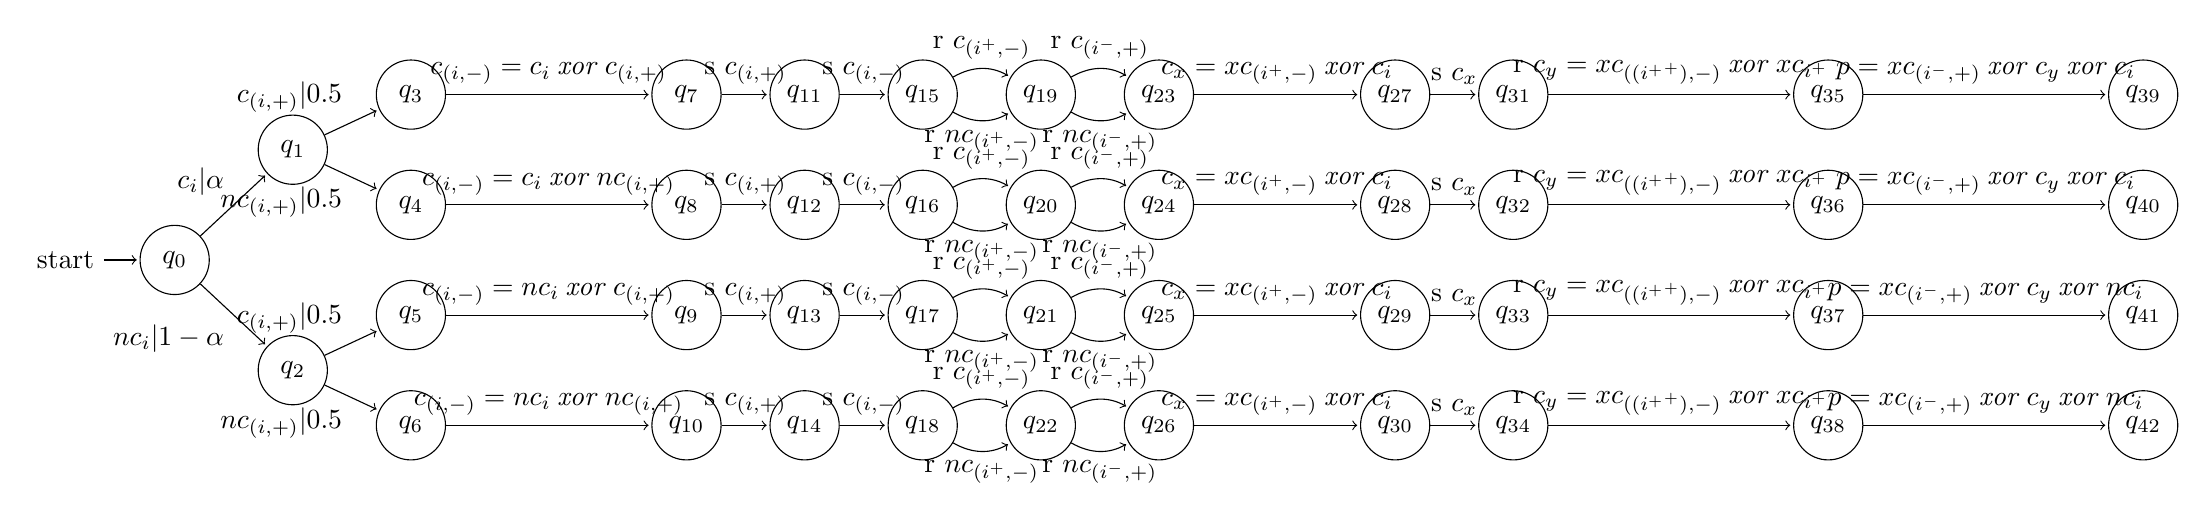
\begin{tikzpicture}[shorten >=1pt,node distance=1.5cm,on grid,auto] 
	\node[state,initial] (q_0)   {$q_0$}; 
	\node[state] (q_1) [above right=1.4cm and 1.5cm of q_0] {$q_1$}; 
	\node[state] (q_2) [below right=1.4cm and 1.5cm of q_0] {$q_2$}; 
	\node[state] (q_3) [above right=0.7cm and 1.5cm of q_1] {$q_3$}; 
	\node[state] (q_6) [below right=0.7cm and 1.5cm of q_2] {$q_6$}; 
	\node[state] (q_4) [below right=0.7cm and 1.5cm of q_1] {$q_4$}; 
	\node[state] (q_5) [above right=0.7cm and 1.5cm of q_2] {$q_5$}; 
	\path[->] 
	(q_0) edge  node {$c_i | \alpha$} (q_1)
	edge  node [swap] {$nc_i | 1 - \alpha$} (q_2)
	(q_1) edge  node {$c_{(i,+)} | 0.5$} (q_3)
	edge  node [swap] {$nc_{(i,+)} | 0.5$} (q_4)
	(q_2) edge  node {$c_{(i,+)} | 0.5$} (q_5)
	edge  node [swap] {$nc_{(i,+)} | 0.5$} (q_6);
	
	\node[state] (q_7) [right=3.5cm of q_3] {$q_7$};
	\node[state] (q_8) [right=3.5cm of q_4] {$q_8$};
	\node[state] (q_9) [right=3.5cm of q_5] {$q_9$};
	\node[state] (q_{10}) [right=3.5cm of q_6] {$q_{10}$}; 
	\node[state] (q_{11}) [right=of q_7] {$q_{11}$}; 
	\node[state] (q_{12}) [right=of q_8] {$q_{12}$};
	\node[state] (q_{13}) [right=of q_9] {$q_{13}$};
	\node[state] (q_{14}) [right=of q_{10}] {$q_{14}$};
	\node[state] (q_{15}) [right=of q_{11}] {$q_{15}$}; 
	\node[state] (q_{16}) [right=of q_{12}] {$q_{16}$};
	\node[state] (q_{17}) [right=of q_{13}] {$q_{17}$};
	\node[state] (q_{18}) [right=of q_{14}] {$q_{18}$};
	\node[state] (q_{19}) [right=of q_{15}] {$q_{19}$}; 
	\node[state] (q_{20}) [right=of q_{16}] {$q_{20}$}; 
	\node[state] (q_{21}) [right=of q_{17}] {$q_{21}$}; 
	\node[state] (q_{22}) [right=of q_{18}] {$q_{22}$}; 
	\node[state] (q_{23}) [right=of q_{19}] {$q_{23}$}; 
	\node[state] (q_{24}) [right=of q_{20}] {$q_{24}$}; 
	\node[state] (q_{25}) [right=of q_{21}] {$q_{25}$}; 
	\node[state] (q_{26}) [right=of q_{22}] {$q_{26}$}; 
      \node[state] (q_{27}) [right=3cm of q_{23}] {$q_{27}$}; 
      \node[state] (q_{28}) [right=3cm of q_{24}] {$q_{28}$}; 
      \node[state] (q_{29}) [right=3cm of q_{25}] {$q_{29}$}; 
      \node[state] (q_{30}) [right=3cm of q_{26}] {$q_{30}$}; 
	\node[state] (q_{31}) [right=of q_{27}] {$q_{31}$}; 
	\node[state] (q_{32}) [right=of q_{28}] {$q_{32}$}; 
	\node[state] (q_{33}) [right=of q_{29}] {$q_{33}$}; 
	\node[state] (q_{34}) [right=of q_{30}] {$q_{34}$}; 
	\node[state] (q_{35}) [right=4cm of q_{31}] {$q_{35}$}; 
	\node[state] (q_{36}) [right=4cm of q_{32}] {$q_{36}$}; 
	\node[state] (q_{37}) [right=4cm of q_{33}] {$q_{37}$}; 
	\node[state] (q_{38}) [right=4cm of q_{34}] {$q_{38}$}; 
	\node[state] (q_{39}) [right=4cm of q_{35}] {$q_{39}$}; 
	\node[state] (q_{40}) [right=4cm of q_{36}] {$q_{40}$}; 
	\node[state] (q_{41}) [right=4cm of q_{37}] {$q_{41}$}; 
	\node[state] (q_{42}) [right=4cm of q_{38}] {$q_{42}$}; 
	\path[->] 
	(q_3) edge  node {$c_{(i,-)}=c_i \xor c_{(i,+)}$} (q_7)
	(q_4) edge  node {$c_{(i,-)}=c_i \xor nc_{(i,+)}$} (q_8)
	(q_5) edge  node {$c_{(i,-)}=nc_i \xor c_{(i,+)}$} (q_9)
	(q_6) edge  node {$c_{(i,-)}=nc_i \xor nc_{(i,+)}$} (q_{10})
	(q_7) edge  node {s $c_{(i,+)}$} (q_{11})
	(q_8) edge  node {s $c_{(i,+)}$} (q_{12})
	(q_9) edge  node {s $c_{(i,+)}$} (q_{13})
	(q_{10}) edge  node {s $c_{(i,+)}$} (q_{14})
	(q_{11}) edge  node {s $c_{(i,-)}$} (q_{15})
	(q_{12}) edge  node {s $c_{(i,-)}$} (q_{16})
	(q_{13}) edge  node {s $c_{(i,-)}$} (q_{17})
	(q_{14}) edge  node {s $c_{(i,-)}$} (q_{18})
	(q_{15}) edge[bend left]  node {r $c_{(i^+,-)}$} (q_{19})
	(q_{15}) edge[bend right]  node[swap] {r $nc_{(i^+,-)}$} (q_{19})
	(q_{16}) edge[bend left]  node {r $c_{(i^+,-)}$} (q_{20})
	(q_{16}) edge[bend right]  node[swap] {r $nc_{(i^+,-)}$} (q_{20})
	(q_{17}) edge[bend left]  node {r $c_{(i^+,-)}$} (q_{21})
	(q_{17}) edge[bend right]  node[swap] {r $nc_{(i^+,-)}$} (q_{21})
	(q_{18}) edge[bend left]  node {r $c_{(i^+,-)}$} (q_{22})
	(q_{18}) edge[bend right]  node[swap] {r $nc_{(i^+,-)}$} (q_{22})
	(q_{19}) edge[bend left]  node {r $c_{(i^-,+)}$} (q_{23})
	(q_{19}) edge[bend right]  node[swap] {r $nc_{(i^-,+)}$} (q_{23})
	(q_{20}) edge[bend left]  node {r $c_{(i^-,+)}$} (q_{24})
	(q_{20}) edge[bend right]  node[swap] {r $nc_{(i^-,+)}$} (q_{24})
	(q_{21}) edge[bend left]  node {r $c_{(i^-,+)}$} (q_{25})
	(q_{21}) edge[bend right]  node[swap] {r $nc_{(i^-,+)}$} (q_{25})
	(q_{22}) edge[bend left]  node {r $c_{(i^-,+)}$} (q_{26})
	(q_{22}) edge[bend right]  node[swap] {r $nc_{(i^-,+)}$} (q_{26})
      (q_{23}) edge  node {$c_x=xc_{(i^+,-)} \xor c_i$} (q_{27})
      (q_{24}) edge  node {$c_x=xc_{(i^+,-)} \xor c_i$} (q_{28})
      (q_{25}) edge  node {$c_x=xc_{(i^+,-)} \xor c_i$} (q_{29})
      (q_{26}) edge  node {$c_x=xc_{(i^+,-)} \xor c_i$} (q_{30})
      (q_{27}) edge  node {s $c_x$} (q_{31})
       (q_{28}) edge  node {s $c_x$} (q_{32})
       (q_{29}) edge  node {s $c_x$} (q_{33})
       (q_{30}) edge  node {s $c_x$} (q_{34})
       (q_{31}) edge  node {r $c_y=xc_{(({i^+}^+),-)} \xor xc_{i^+}$} (q_{35})
       (q_{32}) edge  node {r $c_y=xc_{(({i^+}^+),-)} \xor xc_{i^+}$} (q_{36})
       (q_{33}) edge  node {r $c_y=xc_{(({i^+}^+),-)} \xor xc_{i^+}$} (q_{37})
       (q_{34}) edge  node {r $c_y=xc_{(({i^+}^+),-)} \xor xc_{i^+}$} (q_{38})
       (q_{35}) edge  node {$p=xc_{(i^-,+)} \xor c_y \xor c_i$} (q_{39})
       (q_{36}) edge  node {$p=xc_{(i^-,+)} \xor c_y \xor c_i$} (q_{40})
       (q_{37}) edge  node {$p=xc_{(i^-,+)} \xor c_y \xor nc_i$} (q_{41})
       (q_{38}) edge  node {$p=xc_{(i^-,+)} \xor c_y \xor nc_i$} (q_{42});

	\end{tikzpicture}
	\end{adjustbox}
	\caption{Altruistic player in probabilistic secret sharing}\label{fig:altruistic}
\end{figure*}

\paragraph{Without Byzantine}
Similarly, we show that in each of the above classes, the expected pay-off of any altruistic play is $0$. For example, in the first class -- unique winner and the winner plays $0$, there are $3$ cases: $p_1$ wins, $p_2$ wins, or $p_3$ wins. An altruistic player $p_1$'s pay-offs are $2$, $-1$ and $-1$ respectively. In this class the probability of each outcome is the same. Thus, the expected pay-off of $p_1$ is $0$. Similarly, other players' pay-offs are $0$ in the first class as well. The expected pay-offs of any altruistic player is $0$ in other classes. Therefore,  considering all the classes, the expected pay-off of any altruistic player is $0$. %altruistic player's expected pay-off is $\frac{1}{5} \times \frac{3}{5} \times \frac{3}{5} = \frac{9}{125}$. The probability weighted outcome is $\frac{9}{125} \times (2 + -1 + -1)=0$.
%So, $U_1(\langle s_1^a,s_1^b,s_1^a  \rangle )=0$ in this scenario. 

Next, we calculate the expected pay-off of a rational player using a similar way as in the equal probability strategy. 
Assuming $p_1$ is rational, given that $p_1$ plays rock, there are $9$ outcomes. The pay-off of each outcome is shown in Table~\ref{tab:1}. However, the probability of each outcome is unequal. We calculate the probabilities for each outcome and obtain the expected pay-off of $p_1$ is $0.8$, and calculate the probability of restarting the game as $\frac{86}{125}$. Hence, for each iteration, the expected pay-off of $p_1$ is no less than $0.8$. If any other action of $p_1$ leads to a pay-off less than $0.8$, $p_1$ will play rock instead of the action for achieving better pay-off. Hence, the expected pay-off of $p_1$ in each iteration is no less than $0.8$. For infinite number of iterations, the expected pay-off 
of $p_1$ is obviously larger than $0$. This implies that $V_1(\langle s_1^r,s_1^a,s_1^a  \rangle ) > U_1(\langle s_1^a,s_1^a,s_1^a  \rangle )$. Therefore, the strategy $\langle \frac{1}{5},\frac{1}{5},\frac{3}{5} \rangle$ is NOT a Nash-equilibrium, when there is no Byzantine player.

\paragraph{With one Byzantine player}
Assume player $p_1$ is Byzantine, unlike the case with equal probability strategy,
the unequal probability strategy provides interesting and counter-intuitive scenarios.
We cannot simply consider one iteration and derive the Nash-equilibrium by extending it to multiple iterations.
Essentially, the probability of ending the game plays more important role in the calculation. An action of rational player which leads to bigger pay-off than other actions in one iteration may not always lead to a bigger pay-off in the long run, in the case that the action leads to a significant larger probability to restart the game. For example, in the case that the pay-off is negative, if player's pay-off in the long run is smaller than the pay-off in one iteration then the action that has smaller pay-off in one iteration has larger pay-off in the long run.\\
In the algorithm, $U_i(\langle s_1^b,s_1^a,s_1^a  \rangle,iter)$ was approximately equal to $\frac{-10}{11}$ when $p_2$ is altruistic and $V_i(\langle s_1^b,s_1^r,s_1^a \rangle,iter)$ was approximately equal to $\frac{-5}{3}$ when $p_2$ was rational. The algorithm terminated by returning the result $PASS$. It shows that the strategy  $\langle \frac{1}{5},\frac{1}{5},\frac{3}{5} \rangle$ is a Nash-equilibrium, when $p_1$ is Byzantine. Due to space limitations we do not present the proofs in the paper. Please refer to \cite{Full-version} for proofs.
%A rational player determines her optimal action for the first game, given the optimum cumulative expected pay-off obtained in  subsequent games. Across the iterations of the algorithm, number of these subsequent games is increased. Since 


%For example,

%Assume player $p_1$ is Byzantine, we calculate altruistic player $p_2$'s expected pay-off for a single iteration. Given Byzantine player plays rock, the expected pay-off of $p_2$ is $-0.4$. Similarly, we calculate the pay-off of $p_2$ when $p_1$ plays the other two actions. This is the minimum expected pay-off achieved by player $1$ within a single iteration.Restarting probability is $\frac{14}{25}$. Long-term expected pay-off is $U_1(\langle s_1^a,s_1^b,s_1^a  \rangle )=\frac{-10}{11}$. \\
%When the player $2$ is Byzantine and player $1$ is rational, It can be shown that for the moves $R$ , $P$ and $S$ by player $1$, corresponding Byzantine moves are $P$, $S$ and $R$. The player $1$'s maximum expected pay-off for a single iteration is $\frac{-3}{5}$ and it happens when player $1$ plays $R$. For this strategy of player $1$ and player $2$, probability of restarting is $\frac{4}{5}$. However, there is an interesting fact arising here. The player $1$'s best strategy in a single iteration may not give the maximum guaranteed expected pay off in the long run because, the restarting probabilities are different for each strategy. Lower expected pay-off in a single iteration may produce a higher long-term expected pay-off due to a sufficiently low restarting probability. In this scenario, Strategy $S$ by player $1$ gives the maximum long-term guaranteed expected pay-off $-1 \times \frac{1}{1 - \frac{2}{2}}=\frac{-5}{3}$. Since, $\frac{-10}{11} \geq \frac{-5}{3}$\\
%$U_1(\langle s_1^a,s_1^b,s_1^a  \rangle ) \geq V_1(\langle s_1^r,s_1^b,s_1^a  \rangle ) $. Hence, this constitutes a Nash-equilibrium.

%$C ^ \sharp$ Implementation was able to calculate the approximated long-term utility values allowing error not more than $10^{-4}$.

\subsection{Probabilistic secret sharing}
Secret sharing is a way for a group of users to share a secret: the secret is divided into many parts, named \emph{shares}, and each user in the group has a share; the secret can only be reconstructed with a sufficient number (threshold $m$) of shares. In other words, the secret is kept confidential, even in the presence of a limited number of traitors (compromised users or non-cooperating members who prevent the reconstruction of the secret). This property makes secret sharing an ideal scheme for storing highly sensitive information, such as encryption keys and launch codes. In the parametric form, a $n\mbox{-}m$ ($n\geq m$) secret sharing ensures that it requires at least $m$ altruistic players to reconstruct the secret within a group of $n$ players. That is, less than $m$ compromised players together cannot reconstruct the secret; and less than $n-m$ non-cooperating members together cannot stop the altruistic players from reconstructing the secret.

The most well-known secret sharing scheme is the Shamir's secret sharing~\cite{Shamir79}. However, the scheme does not work when the players are rational. It is shown that a rational player will not share her secret with anyone else ~\cite{HT04}. In fact, it is proved that in general, in all practical mechanisms for shared-secret reconstruction with an upper bound on the running time, the best strategy for each rational player is to deviate from the specification by doing nothing~\cite{HT04}. Hence, a randomized mechanism (the probabilistic secret sharing scheme) is proposed to ensure that rational players would reveal their shares to reconstruct the secret, i.e., achieving a Nash-equilibrium with a constant expected running time. 

\subsubsection{Protocol description}
The probabilistic scheme is a $3\mbox{-}3$ secret sharing. 
Given the $3$ players, we index each player with a distinct number in $\{1, 2, 3\}$. We use $i$ to denote one player, then the other two players are $(i+1)\%3$, denoted as $i^+$, and $(i-1)\%3$, denoted as $i^-$. There is an issuer who assigns each player a share of secret. Assuming the share cannot be changed; for example, it is signed by the issuer.
The scheme works as follows.
\begin{enumerate}
\item Each player $i$
\begin{itemize}
\item chooses a bit $c_i$ ($c_i$ can only be $1$ or $0$) such that $c_i =1$ with probability $\alpha$ and $c_i = 0$ with probability $1-\alpha$; 
\item chooses a bit $c_{(i,+)}$ ($c_{(i,+)}$ can only be $1$ or $0$) randomly, so that $c_{(i,+)}=1$ with probability $1/2$ and $c_{(i,+)}=0$ with probability $1/2$;
\item calculates $c_{(i,-)}= c_i \xor c_{(i,+)}$. 
\end{itemize}
Then player $i$ sends the bit $c_{(i,+)}$ to player $i^+$ and sends the bit $c_{(i,-)}$ to player $i^-$. This means that the player $i$ receives a bit $c_{(i^+,-)}$ from player $i^+$ and a bit $c_{(i^-,+)}$ from player $i^-$.
\item On receiving $c_{(i^+,-)}$, player $i$ computes $c_{(i^+,-)} \xor c_i$ and sends it to player $i^-$. Correspondingly, $i$ receives $c_{((i^+)^+, -)} \xor\ c_{i^+}$ from $i^+$. Since there are only $3$ players, player $(i^+)^+$ is the player $i^-$. Hence $c_{((i^+)^+, -)} \xor c_{i^+}=c_{(i^-,-)} \xor c_{i^+}$.
\item When receiving both $c_{(i^-,+)}$ from player $i^-$ (step 1) and receiving $c_{(i^-,-)} \xor c_{i^+}$ from $i^+$ (step 2), $i$ computes $p = c_{(i^-,+)} \xor (c_{(i^-,-)}\xor c_{i^+})\xor c_i$. Note that $ c_{(i^-,+)} \xor (c_{(i^-,-)}\xor c_{i^+})\xor c_i=c_{i^-} \xor c_{i^+}\xor c_i$, i.e., $p=c_1 \xor c_2 \xor c_3$ (It holds for all players).
If $p = c_i = 1$ then player $i$ sends her share to the others.
\item Depending on the value of $p$ and the shares received, player $i$ constructs the secret, restarts the protocol or reports cheating.
\begin{itemize}
\item If $p=1$, $i$ receives $3$ shares, then he construct the secret.
\item If $p =0$ and $i$ received no secret shares, or if $p =1$ and $i$ received exactly one share (possibly from itself; that is, we allow the case that $i$ did not receive any shares from other players but sent its own), the issuer restarts the protocol. 
\item Otherwise, player $i$ stops the protocol. Because someone must have been cheating. 
\end{itemize}
The intuition behind the last step is as follows: When $p=0$, no one should send her share; and thus $i$ receives no secret share. Otherwise, someone calculated wrong (cheating).
When $p=1$ either $c_i=c_{i^+}=c_{i^-}=1$ or there exists exactly one player chooses $1$, i.e., $c_i=c_{i^+}=0$ and $c_{i^-}=1$, $c_i=c_{i^-}=0$ and $c_{i^+}=1$, or $c_{i^+}=c_{i^-}=0$ and $c_i=1$. 
In the former case, each player can construct the secret. In the later case, $i$ should receive exactly one share then the issuer restarts the protocol. Otherwise, some player calculated wrong (cheating). 
\end{enumerate}


\subsubsection{Modelling}
The model of the altruistic players who follow the protocol specification is straightforward.
For the sake of space saving, we present the FMS for altruistic players in the graphical manner as
in Figure~\ref{fig:altruistic}. In the Figure, we use `s' to stand for sending and `r' to stand for receiving,
use $nc_i$ to represent the opposite value of $c_i$; the value after symbol $|$ is the probability of the action, for example, $c_i|\alpha$ stands for that the probability of choosing the value $c_i$ is $\alpha$. For simplicity of presentation, we merged the states and traces caused by
received values and use the prefix $xc$ to represent either $c$ or $nc$ depending on which one is received.
The payoff function is defined as follows: \\
$\shia(\gs)=\left\{\begin{array}{ll}
3 & \mbox{if only the player \textit{i} gets secret}\\
2 &\mbox{if the player \textit{i} and another player get secret}\\
1 &\mbox{if everyone knows the secret}\\
0 &\mbox{if no one knows the secret}\\
-1 & \mbox{if other two players know the secret} \\
-2 & \mbox{if only one other player knows the secret} 
\end{array}\right. $
%
The Byzantine players deviate from the protocol specification by sending the opposite 
value of the one that the player should send. For example, in a Byzantine player's model,
we add a transition from $q_7$ to $q'_{11}$ labelled with $nc_{(i,+)}$, and copy the transition
from $q_{11}$ to $q_{39}$ as $q'_{11}$ to $q'_{39}$. Similar for other states which enables
sending actions. Due to space limit, we omit the figure for Byzantine players.
The model of rational players are the model of Byzantine players together with the above pay-off function.

Notice that we fixed the order of all players' sending and receiving actions such that 
the three players' sending and receiving actions can be synchronised. That is, we
did not model the full interleaving of all the possible 
orders of sending and receiving actions of the three players. We show that this does
not influence the verification result.

\subsubsection{Verification results}
We verified whether a player deviates from the specification in two settings: without Byzantine player and
with one Byzantine player. 
Essentially, our algorithm calculates the pay-off of a player in the following four configurations and compare the pay-offs.
\begin{enumerate}
	\item All the three players are altruistic ($m=0$)
	\item Two players are altruistic and one player is rational ($m=0$)
	\item Two players are altruistic and one player is Byzantine ($m=1$)
	\item One player is altruistic, one player is Byzantine and one player is rational ($m=1$)
\end{enumerate}
The verification result shows that the probabilistic secret sharing protocol is a Nash-equilibrium when there is no Byzantine player,
which confirms the manual analysis in its original paper. In addition, the verification
result shows that even with a Byzantine player, the probabilistic secret sharing scheme is 
still a Nash-equilibrium, which has not been proved in existing works.





 
%$W_i^{t}(s)=\left\{\begin{array}{l}
%0\ \mbox{if}\ t=0\\
%E(SH_i(s')+W_i^{t-1}(s')| T(s,a)=s' \text{ for some a})\\
%\end{array}\right. $
% It is sufficient to prove that $|W_i^{t}(s)|$ is increasing w.r.t. $t$, $s \in S$ and $i \in [n]$ and $|W_i^{t}(s)|$ is bounded below by
%  $\frac{N \times max_s\{|SH_i(s)| \}}{p_{min}^{N}}$.



\section{Examples}\label{sec:ex}
It appears that the optimal move for a single iteration optimizes the expected pay-off in the long run. We have proved that for equal probability strategy, optimal moves for rational player and Byzantine player was the repetitive use of optimal move for each single iteration. For unequal probability strategy without Byzantine player we do not have to consider the optimal long-run strategy of a rational player to prove the Nash-equilibrium. (The reason is that optimal long-run expected pay-off for an altruistic player is $0$ irrespective of the strategy, and the rational player has a strategy which results in a positive pay-off for each iteration. It is logical that optimal strategy of the rational player also results in a positive expected pay-off. In order to arrive at this conclusion we do not explicitly generate the optimal rational strategy.)  When it comes to unequal probability strategy with Byzantine players, we need to calculate optimal strategies for rational players as well as altruistic players because, we do not have any logical inferencing to argue about the optimal long-run expected pay-offs without explicitly generating them. Now, the claim about repeating the move which optimized a single iteration to optimize the expected pay-off in the long-run, has become counter intuitive. We start by investigating the case where, we have unequal probability strategy with Byzantine player for a game having two iterations.\\
The analysis considers the case when $p_1$ is Byzantine, $p_2$ is rational and $p_3$ is altruistic. $p_1$,$p_2$ and $p_3$ are defined in section \ref{sec:casestudy}.
We define following $6$ symbols. $\gamma_0$, $\gamma_1$ and $\gamma_2$ are the restarting probabilities when $p_2$ plays rock , paper , scissor moves respectively. $X_0$, $X_1$ and $X_2$ are the expected pay-offs for $p_2$ , for rock , paper , scissor moves respectively.
$\gamma_0=\frac{4}{5}$, $\gamma_1=\frac{4}{5}$ and $\gamma_2=\frac{2}{5}$.\\
We show the calculation for $X_0$ here. 
Table \ref{tab:3} shows the pay-offs for a rational player in a single iteration when he plays rock. According to the table, expected pay-off for the first iteration is calculated as,\\
$\frac{1}{5}\times (-1) + \frac{1}{5}\times (-2) + \frac{3}{5}\times (-0) = \frac{-3}{5}$. Hence, $X_0=\frac{-3}{5}$. $X_1$ and $X_2$ are calculated in a similar way. The results are $X_1=\frac{-7}{5}$ and $X_2=-1$ respectively.\\
Consider two iterations, the expected pay-off for rational player $p_2$ in two iterations is calculated as, \\
$X_i+P_i\times X_j$ where $i,j \in \{0,1,2\}$. Since $\gamma_0=\gamma_1$ and $X_0 > X_1$, rock move is more optimal than paper move in both iterations. Hence, we consider only the rock move and the scissor move for the analysis. Now we have four strategies to compare. (two moves for the first iteration $\times$ two moves for the second iteration) For any given first move, the second move to optimize the summation would be the maximum between $X_0$ and $X_2$. Now we have only two strategies to compare.\\
\begin{itemize}
	\item $X_0+\gamma_0\times X_0= \frac{-3}{5} + \frac{4}{5}\times \frac{-3}{5}=-1.44 $\\
	\item $X_2+\gamma_1\times X_0= -1 + \frac{2}{5}\times \frac{-3}{5}=-1.24$
\end{itemize}
We can see that second strategy becomes optimal as instead of repetitive rock strategy. This counter intuitive result is caused by the restarting probability. In case of negative pay-offs, even though a move has high expected pay-off values in a single iteration, higher restarting probabilities make them less profitable in the long-run and vice-versa.\\
 We can deduce that the long-run optimal altruistic and rational strategies for an infinite number of iterations is not trivial. We show how to determine the optimal strategies in the long-run in our proof of Nash-equilibrium for the unequal strategy in Section \ref{sec:proofs}.
\section{Theorems and Proofs}\label{sec:proofs}

\begin{theorem}\label{thm: NE}
	Let $\mathcal{M}$ be a mechanism defined in section \ref{sec:ex}.
	Let $\pia(s^a_1, 0) = 1/5, \pia(s^a_1, 1)= 1/5, \pia(s^a_1, 2) = 3/5$. Suppose there is one Byzantine player. $\pia$ is a Nash-equilibrium
\end{theorem}

First we have to show that, rational players strategy is always playing the scissor move. 

We use the notation defined in section \ref{sec:ex} for the rest of the proof.
To calculate the expected pay-off for the rational player in the long-run, we have to define restarting probabilities and expected pay-offs w.r.t. each iteration. For the $i^{th}$ iteration there is a corresponding $X^{(i)}$ term and a $P^{(i)}$ term. $X^{(i)}$ is the expected pay-off at $i^{th}$ iteration. $X^{(i)}$ can take any value among $\{ X_0, X_1, X_2 \}$.\\ $P^{(i)}$ is the restarting probability at $i^{th}$ iteration. $P^{(i)}$ can take any value among $\{ \gamma_0, \gamma_1, \gamma_2 \}$. Since the restarting probability depends on the current move, $X^{(i)}$ and $P^{(i)}$ can be related. \\
$\forall$ $k \in$ $\{0,1,2\}$, $X^{(i)}=X_k \iff P^{(i)}=P_k $ 
Now we can define the weighted expected pay-off of the iteration $i$. Simply it should be the product of expected pay-off of the iteration $i$ and the probability of reaching iteration $i$.\\
Expected pay-off of the iteration $i$ is $X^{(i)}$. probability of reaching iteration $i$ is\\

$Pr(i)=\left\{\begin{array}{l}
1\ \mbox{if}\ i=1\\
\Pi_{k=1}^{i-1}P^{(k)} \ \mbox{if}\ i>1\\
\end{array}\right. $

The long run pay-off is the infinite summation of all the weighted expected pay-offs is,\\

$\Sigma_{i=1}^{\infty} X^{(i)}Pr(i)$.\\

\begin{lemma}\label{lem:conv}
	The series  $\Sigma_{i=1}^{\infty} X^{(i)}Pr(i)$ Converges.
\end{lemma}
\begin{proof}
	We can prove the absolute convergence of  the series which is sufficient to prove the convergence of the original series. \\
	$\Sigma_{i=1}^{\infty} |X^{(i)}Pr(i)|$\\
	$\impliedby \Sigma_{i=1}^{\infty} |X^{(i)}||Pr(i)|$ \\
	Let's consider the summation of $n$ terms in the series ($\Sigma_{i=1}^{n} |X^{(i)}||Pr(i)|$) as the $n^{th}$ term in a sequence. Then we have to prove the convergence of this sequence. According to  sequence convergence theorems we can prove that the sequence is increasing and bounded above. Increasing property is trivial because the series has absolute values.\\
	$|X^{(i)}| < c=max(\{ |X_0|, |X_1|, |X_2| \}) \forall$ $i$\\
	$|P^{(i)}| < q=max(\{ |\gamma_0|, |\gamma_1|, |\gamma_2| \}) \forall$ $i$\\
	$|Pr(i)| < q^{i-1} \forall$ $i$\\
	$\Sigma_{i=1}^{\infty} |X^{(i)}Pr(i)| \le \Sigma_{i=1}^{\infty} cq^{i-1}$\\
	The right hand side of the inequality shows an infinite geometric progression with the common-ratio $q$ and the initial term $c$. Since, $q < 1$ this series converges to $\frac{c}{1-q}$. \\
	$\Sigma_{i=1}^{\infty} |X^{(i)}Pr(i)| \le \frac{c}{1-q}$.\\
	$\Sigma_{i=1}^{n} |X^{(i)}Pr(i)| \le \frac{c}{1-q}$ $\forall n$. \\
	The sequence $\Sigma_{i=1}^{n} |X^{(i)}Pr(i)|$ is bounded above. Hence The series,\\
	$\Sigma_{i=1}^{\infty} |X^{(i)}Pr(i)|$ converges. The absolute convergence implies the convergence of the original series as well.
\end{proof}

\begin{proof}(Theorem \ref{thm: NE})
 
 
 Now we can proceed with our optimality proof. We first have a general strategy $Sr$ and $Sr=\Sigma_{i=1}^{\infty} X^{(i)}Pr(i)$. The value $Sr$ exists as a real number by lemma \ref{lem:conv}. For the sake of argument\\
 let  $\exists j $ s.t. $X^{(j)}=X_2$. Now define $Sr_0$ to be the long-run pay-off achieved by changing the scissor move at iteration $j$, to a rock move. Also define  $Sr_1$ to be the long-run pay-off achieved by changing the scissor move at iteration $j$ to a paper move. If we prove that $Sr_0-Sr<0$ and $Sr_1-Sr<0$ then it is evident that playing scissors at any iteration is optimal.\\
 
 \begin{itemize}
 	\item Case $1$: Proof of $Sr_0-Sr<0$\\
 	It is clear that terms in the both series appear before $j^{th}$ term cancels off when finding the difference. Let $j^{th}$ term of the series $Sr$ and $Sr_0$ are $Sr(j)$ and $Sr_0(j)$ respectively.\\
 	$Sr_0-Sr=\Sigma_{i=j}^{\infty} Sr_0(i) - Sr(i)$.\\
 	$Sr_0(j) - Sr(j)=Pr(j)(X_0-X_2)$. Let $M=\Sigma_{i=j+1}^{\infty}Sr(i)$. With the change of move in $j^{th}$ iteration, for every product $Pr(i), i > j$ $P^{j}$ is changed from $\gamma_2$ to $\gamma_0$. $\Sigma_{i=j+1}^{\infty}Sr_0(i)= \frac{\gamma_0}{\gamma_2}M$.\\
 	$\Sigma_{i=j+1}^{\infty} Sr_0(i) - Sr(i)=\frac{\gamma_0}{\gamma_2}M-M$.\\
 	$Sr_0-Sr=Pr(j)(X_0-X_2)+\frac{P_0}{P_2}M-M$.\\
 	Let's substitute the known values the expression,\\
 	$Pr(j)(\frac{-3}{5} - (-1))$ $+ \frac{\frac{4}{5}}{\frac{2}{5}}\times M - M$.\\
 	Now it is sufficient to prove that,
 	$Pr(j)\frac{2}{5} + M < 0$\\
 	$\impliedby |M| > Pr(j)\frac{2}{5}$. ($M < 0$)\\
 	By dividing both sides of the inequality by $Pr(j)$, Left hand side of the inequality becomes,\\
 	$M'=\Sigma_{i=j+1}^{\infty} (\Pi_{k=j}^{i-1}P^{(k)})X^{(i)}$ \\
 	$\impliedby |M'| > \frac{2}{5}$ . Now we find a lower bound for $M'$ and prove that it is always greater than $\frac{2}{5}$.  To find the lower bound we substitute the least absolute value among $\{X_0,X_1,X_2\}$ and $\{\gamma_0,\gamma_1,\gamma_2\}$ which would be  	$\frac{3}{5}$ and $\frac{2}{5}$ respectively to all the $X^{(i)}$'s and $P^{(i)}$'s. So, $M'$ reduces to the geometric progression,\\
 	$\frac{3}{5}(\frac{2}{5}+\frac{2}{5}^2+ \dots)$. Which converges to $\frac{2}{5}$. The finite summation for any number of terms in $|M'|$ is always $< \frac{2}{5}$. Now we can see that this lower bound is not sufficient to prove that $|M'| > \frac{2}{5}$ for sufficiently large number of terms in the series\\
 	However, we know that the above substituted values do not show an existing path for a rational player. To arrive at an existing path we have to change at least one substituted value of $X^{(i)}$'s or $P^{(i)}$'s. Let's say this substitution increases the converged value by $\epsilon$. According to series convergence theorems we can also find $\epsilon' < \epsilon$ s.t $|M'| > \frac{2}{5} - \epsilon'$ for a finite summation of sufficiently large number of terms. After the new substitution, $|M'|$ becomes $M''=|M'|+\epsilon$. (the convergence can be proven)\\
 	$|M'|+\epsilon > \frac{2}{5} - \epsilon' + \epsilon$ \\
 	$\implies M'' > \frac{2}{5}$ for a sufficiently large number of terms.\\
 	$\implies |M| > \frac{2}{5}$ for a sufficiently large number of terms.
 	\item Case $2$: Proof of $Sr_1-Sr<0$\\
 	After substitution Case $2$ reduces to prove that\\
 	$Sr_1-Sr=Pr(j)(X_1-X_2)+\frac{\gamma_1}{\gamma_2}M-M < 0$. Now let's substitute the values to the expression it is sufficient to prove that .\\
 	$Pr(j)(\frac{-2}{5}) + M < 0$ which is obvious because $M < 0$.
 \end{itemize}
 
 According to the best strategy of the rational player which is proven above, the optimal expected pay-off in the long-run for the rational player is $\frac{-5}{3}$.
 
 Now we can prove the best strategy for an altruistic player. In this scenario we have two altruistic players and one Byzantine player. We have to consider the pay-offs for each move of the Byzantine player. We are going to prove that Byzantine playing  rock at each iteration results in the worst outcome for an altruistic player. \\
 Values for $\gamma_0$ , $\gamma_1$ and $\gamma_2$ become $\frac{14}{25}$, $\frac{18}{25}$ and $\frac{18}{25}$ respectively. $X_0$ , $X_1$ and $X_2$ become $-0.4$, $0.4$ and $0$ respectively.\\
 Similar to the previous proof, we can name the general expression for the cumulative expected pay off in long-run as $Sr$. The expression results in modifying rock move to paper move and scissor move are named as $Sr_1$ and $Sr_2$ respectively. $Sr_1$ and $Sr_2$ also exist by lemma \ref{lem:conv}.
 What we have to prove is $Sr_1 - Sr > 0$ and $Sr_2 - Sr > 0$.\\
 
 \begin{itemize}
 	\item Case $1$: Proof of $Sr_1 - Sr > 0$
 	After similar simplification to previous proof, It is left to prove that\\
 	$0.8Pr(j) + \frac{4}{14}M > 0$. Here, each $Pr(j)$ and $M$ have same semantics to previous proof. If $M>0$ the result is trivial. We have to check the result only for the case where $M < 0$. We are going to find an upper bound for $|M|$ when $M<0$. This upper bound occurs when each term of $M$ is negative. For a term of $M$ to be negative, the rock strategy must be followed, because expected pay-offs of other two strategies are non-negative. To result in an upper bound each term in $M$ have to be bounded above. We bound each term of $M$ by substituting $X^{(i)}$ with $X_0=-0.4$ and substituting $P^{(i)}$ with $\frac{18}{25}$ which is the maximum among $\{ \gamma_0, \gamma_1, \gamma_2 \}$. After the substitution, and dividing both sides by $Pr(j)$ we have $M'= \frac{M}{Pr(j)}$\\
 	$|M'| = 0.4(\frac{18}{25}+\frac{18}{25}^2+ \dots)$ This converges to $\frac{36}{35}$. We have to prove that\\
 	$\frac{4}{14}|M'| < 0.8$.By substituting the value of $M'$ we get\\
 	$\frac{72}{245} < 0.8$ \\
 	$\implies 0.8Pr(j) + \frac{4}{14}|M| > 0 $.
 	
 	\item Case $2$: Proof of $Sr_2 - Sr > 0$
 	It is left to prove that $0.4Pr(j) + \frac{4}{14}M > 0$. We can use the same upper bound for $|M|$ as in Case $1$ and the proof reduces to proving,\\
 	$\frac{72}{245} < 0.4$.
 \end{itemize}
 
 The Byzantine player chooses the worst strategy for the altruistic player, which is proven above. The optimal expected pay-off in the long-run for the altruistic player is $\frac{-10}{11}$. \\
 Since $\frac{-10}{11} \ge \frac{-5}{3}$ the altruistic strategy $\langle \frac{1}{5},\frac{1}{5},\frac{3}{5} \rangle$ is a Nash-equilibrium when $p_1$ is Byzantine. 	
\end{proof}

 

 	
% 	We would add all $X^{i}$ s with $C=max(\{ |X_0|, |X_1|, |X_2| \})$ so the resulting series $Sr'$ becomes non negative. The new series is increasing and bounded above by
% 	$Sr' \le \frac{2C}{1-max(\{ P_0, P_1, P_2 \}) }$. Hence $Sr'$ converges.\\
% 	And now consider the series $C'=\Sigma_{i=1}^{\infty} C \times Pr(i)$. This series is also increasing and can be bounded above by $C' \le \frac{C}{1-max(\{ P_0, P_1, P_2 \}) }$. $C'$ also converges.\\
% 	Now $Sr=Sr'-C'$. Since each of $Sr'$ and $C'$ converges $Sr$ also converges.


   
 Now we can prove that the long-run expected pay-off $V_i(init,t)$ and $U_i(init,t)$ (notation in section \ref{sec:verification}) also converge. 
 Let $s^(1),s^(2) \dots$ denote the global state sequence visited during a game execution. If we fix a sequence of valid choices of actions by Byzantine and rational players we obtain a sub graph of the global graph. For example, a valid action choice sequence can be $\langle (rock,paper),(rock,paper),\dots, (rock,paper) \rangle$ where we have one Byzantine player and one rational player.
 
 \begin{defn}
 $Te=\{s | s \in S . \forall$  $a \in A$  $, \forall s' \in S$ $ T(s,a) \neq s' \}$
 \end{defn}
 
 Formally, if a game terminates, $P(\exists i s.t s^(i) \in Te) \rightarrow 1$. Following theorem introduces the condition in global state graph to assure $P(\exists i s.t s^(i) \in Te) \rightarrow 1$. This condition will also assure that the cumulative expected pay-off for any rational player converges.  \\


\begin{theorem}\label{thm:reach}
%	Consider the global graph of the Mechanism $\mathcal{M}$. Introduce an initial state $\hat{x}$ which has a directed transition to each initial state $\in I$. Introduce a terminal state $F$ which is one directed edge away from each of the terminal states.\\
%	If all the non-initial states can be reachable from the initial state $\hat{x}$ and  $F$ also can be reachable by non-terminal in the graph
If for any sequence of valid action choices of Byzantine and rational players,  the corresponding sub graph contains a path from each initial state to a terminal state then  \\
	$P(\exists i s.t s^(i) \in Te) \rightarrow 1$
\end{theorem}


%The reachability properties in the theorem \ref{thm:reach} can be verified by performing a depth first search, 
%\begin{enumerate}
%	\item From initial state $\hat{x}$  on graph $\mathcal{M}$
%	\item From final state $F$ on inverted graph of $\mathcal{M}$
%\end{enumerate}
%Inverted graph, refers to the graph obtained by inverting the edge directions of the original graph.

\begin{proof}(Theorem \ref{thm:reach})
 For a given sub graph corresponding to a sequence of valid action choices of Byzantine and rational players, there is a loop less longest path from an initial state to a terminal state.  Let $N$ be the length of longest of such paths among all the sub graphs corresponding to valid action choices . The minimum probability of reaching a terminal state occurs in the maximal length path. $N$ represents the length of this path. Let's name the minimal probability for a transition as $p_{min}>0$. The minimum probability exists because, the number of probabilistic transitions is finite. The probability of the given $N$ length path ($p_{min}^N$) is a lower bound for reaching any terminal state within $N$ steps. We can extend this to reaching any terminal state within $2N$ steps to $p_{min}^N(1+(1-p_{min}^N))$\\
Reaching a terminal state within $iN$ steps is\\ $p_{min}^N(\Sigma_{k=0}^{i-1}(1-p_{min}^N)^k)$ which becomes an infinite geometric series when $i$ tends to $\infty$. This converges to\\
 $p_{min}^N \times \frac{1}{1-(1-p_{min}^N)}= p_{min}^N \times \frac{1}{(p_{min}^N)}=1$. Since a series which is a lower bound to termination probability converges to probability $1$, and the total probability which is an upper bound to the termination probability converges to probability $1$. The actual termination probability also converges to probability $1$ by sandwich theorem.
\end{proof}


\begin{theorem}
	Let $i$ is an index for a non-Byzantine player according to section \ref{sec:spec}. Let $init \in I$. $V_i$ and $U_i$ are as defined in section \ref{sec:verification}.
	The sequences  $V_i(init,t)$ and $U_i(init,t)$ converge when $t \rightarrow \infty$.
\end{theorem}

\begin{proof}
	We first prove that, cumulative expected pay-off under valid choice of actions of Byzantine and rational players converge. We should write a general expression to represent the cumulative expected pay-off. We denote the global action for the $t^{th}$ step by the variable $x_t$. \\
	
	To visualize the strategy, we present a tree diagram. The tree diagram represents the reachable global states with the actions of the altruistic players when the actions of Byzantine players and rational players are fixed. Probabilities for each branch in the tree diagram are the product of probabilities for each altruistic action which lead to the resulting global state. In other words, branch probability is a joint probability. 
	
	\begin{forest}
		for tree={
			circle,
			draw,
			minimum height=1cm,
			anchor=north,
			align=center,
			child anchor=north
		},
		[{Start}, align=center, name=SS
		[{$S_1$}, name=st1
		[$S_3$, name=st3
		[$T$]
		[$S_6$]
		]
		[{$S_4$}
		[$S_7$]
		[$S_8$]
		]
		]
		[{$S_2$}, name=st2
		[$S_5$, name=st5
		[$S_9$]
		[$S_{10}$]
		]
		[{$T$}]
		]
		]
		%	\node[anchor=west,align=left] 
		%	at ([xshift=-2cm]MS.west) {Level 3\\Criteria};
		%	\node[anchor=west,align=left] 
		%	at ([xshift=-2cm]MS.west|-PDC) {Level 2\\ Group Criteria};
		%	\node[anchor=west,align=left] 
		%	at ([xshift=-2cm]MS.west|-SS) {Level 1\\Overall Objective};
	\end{forest}
	
	Node $Start$ is in level $0$, node $S_1$ and $S_2$ are in level $1$ and so on.
	In the above diagram, first level containing a terminal state is found $2$ steps steps after the starting state and one step after finding the first terminal state, second level containing the terminal state is found. Let's call $n_i$ is the difference (in levels) between $i^{th}$ level with a terminal state and $i-1^{th}$ level with a terminal state for $i>1$ $n_1$ is the level number of the first level containing a terminal state.\\
	Consider the minimum probability of reaching the first terminal state from the starting state which results in the maximum probability of the continuation of the game. Hence the maximum restarting probability after reaching the first terminal state is $(1-p_{min}^{n_1})$. Let $h_{max}= max_s |SH_k(s)|$. Cumulative pay-off value until the first level of termination can be bounded above by,\\
	$n_1 \times h_{max} \times (1-p_{min}^{n_1}) $ Cumulative pay-off value from the first level of termination to the second level of termination can be bounded above by,\\
	$n_2 \times h_{max} \times (1-p_{min}^{n_1})(1-p_{min}^{n_2}) $.\\
	Cumulative pay-off value from the $i-1 ^{th}$ level of termination to the $i^{th}$ level of termination can be bounded above by,\\
	$n_i \times h_{max} \times \Pi_{j=1}^{i} (1-p_{min}^{n_j}) $\\
	The formula for the upper bound of the cumulative pay-off value can be written as,\\
	$\Sigma_{i=1}^{\infty}(n_i \times h_{max} \times \Pi_{j=1}^{i} (1-p_{min}^{n_j})) $
	Since $n_i$, $n_j$ are strategy dependant, we substitute $N$ in the place of $n_i$ and $n_j$ to arrive at an upper bound which matches all the strategies.\\
	$\Sigma_{i=1}^{\infty}(N \times h_{max} \times (1-p_{min}^{N})^i) $\\
	By using the infinite summation for geometric series, the upper bound can be written as,\\
	$\frac{Nh_{max}}{p_{min}^{N}}$\\
	Note that, in the formula for a general strategy we have to substitute the exact expected pay-off value in the place of $n_i \times h_{max}$. We can see that by substituting $h_{max}$ we have also found out that the series for the absolute values of the pay-offs is also bounded above. \\
	Since the absolute pay-off series is a summation of positive values, the summation is an increasing function. This means absolute pay-off series is convergent which implies the actual pay-off series is also convergent.\\
	We proved above, cumulative expected pay-off for any altruistic strategy (Byzantines and rationals are fixed) converges in the long run. The values calculated for $V_i$ and $U_i$ should also converge.
\end{proof}

  
\section{Conclusion}\label{sec:conclusion}
In this article, we presented a framework for probabilistic BAR systems. We introduced an algorithm to verify Nash-equilibrium properties in concurrent games with perfect and imperfect information at the level of global state knowledge. We performed our algorithm on two case studies, the 3-player Rock-Paper-Scissors example and Halpern et al.'s Secret Sharing protocol. Some results are interesting as they illustrate the necessity of a Byzantine player in a game to ``force'' the rational player to behave altruistically notably in the Rock-Paper-Scissors example. This opens a new door for Byzantine players, which are currently only considered as misconfigured or corrupted agents. Our algorithm is guaranteed to terminate (due to the maximum number of iterations) but the convergence may be not guaranteed if $V_i$ and $U_i$ converge to the same value. The analysis of this case is left to future work.
\bibliographystyle{IEEEtran}
\bibliography{iceccs}
\end{document}
